\documentclass[a4paper]{article}
\usepackage[T1]{fontenc}			% \chapter package
\usepackage[english]{babel}
\usepackage[english]{isodate}  		% date format
\usepackage{graphicx}				% manage images
\usepackage{amsfonts}
\usepackage{booktabs}				% high quality tables
\usepackage{amsmath}				% math package
\usepackage{amssymb}				% another math package (e.g. \nexists)
\usepackage{bm}                     % bold math symbols
\usepackage{mathtools}				% emphasize equations
\usepackage{stmaryrd} 				% '\llbracket' and '\rrbracket'
\usepackage{amsthm}					% better theorems
\usepackage{enumitem}				% manage list
\usepackage{pifont}					% nice itemize
\usepackage{cancel}					% cancel math equations
\usepackage{caption}				% custom caption
\usepackage[]{mdframed}				% box text
\usepackage{multirow}				% more lines in a table
\usepackage{textcomp, gensymb}		% degree symbol
\usepackage[x11names]{xcolor}		% RGB color
\usepackage[many]{tcolorbox}		% colorful box
\usepackage{multicol}				% more rows in a table (used for the lists)
\usepackage{listings}
\usepackage{url}
\usepackage{qrcode}
\usepackage{fontawesome5}
\usepackage{ragged2e}
\usepackage{cite}                   % references
\usepackage{imakeidx}               % index
\makeindex[program=makeindex, columns=1,
           title=Index, 
           intoc,
           options={-s index-style.ist}]


\definecolor{codegreen}{rgb}{0,0.6,0}
\definecolor{codegray}{rgb}{0.5,0.5,0.5}
\definecolor{codepurple}{rgb}{0.58,0,0.82}
\definecolor{backcolour}{rgb}{0.95,0.95,0.92}
\lstdefinelanguage{misc}
{
  % list of keywords
  morekeywords={%
    add,
    addi,
    lw,
    sw,
    beq,
    bne,
    j,
    jr,
    offset,
    sub,
    and,
    or
  },
  sensitive=false, % keywords are not case-sensitive
  morecomment=[l]{\#}, % l is for line comment
  % morecomment=[s]{/*}{*/}, % s is for start and end delimiter
  % morestring=[b]" % defines that strings are enclosed in double quotes
}
\lstdefinestyle{mystyle}{
    backgroundcolor=\color{backcolour},   
    commentstyle=\color{codegreen},
    keywordstyle=\color{magenta},
    numberstyle=\tiny\color{codegray},
    stringstyle=\color{codepurple},
    basicstyle=\ttfamily\footnotesize,
    breakatwhitespace=false,         
    breaklines=true,                 
    captionpos=b,                    
    keepspaces=true,                 
    numbers=left,                    
    numbersep=5pt,                  
    showspaces=false,                
    showstringspaces=false,
    showtabs=false,                  
    tabsize=2
}
\lstset{style=mystyle}



% draw a frame around given text
\newcommand{\framedtext}[1]{%
	\par%
	\noindent\fbox{%
		\parbox{\dimexpr\linewidth-2\fboxsep-2\fboxrule}{#1}%
	}%
}


% table of content links
\usepackage{xcolor}
\usepackage[linkcolor=black, citecolor=blue, urlcolor=cyan]{hyperref} % hypertexnames=false
\hypersetup{
	colorlinks=true
}


\newtheorem{theorem}{\textcolor{Red3}{\underline{Theorem}}}
\renewcommand{\qedsymbol}{QED}
\newcommand{\dquotes}[1]{``#1''}
\newcommand{\longline}{\noindent\rule{\textwidth}{0.4pt}}
\newcommand{\circledtext}[1]{\raisebox{.5pt}{\textcircled{\raisebox{-.9pt}{#1}}}}
\newcommand{\definition}[1]{\textcolor{Red3}{\textbf{#1}}\index{#1}}
\newcommand{\example}[1]{\textcolor{Green4}{\textbf{#1}}}
\newcommand{\highspace}{\vspace{1.2em}\noindent}


\begin{document}
    \newcounter{definition}[section]
    \newcounter{example}[section]
    
    \newtcolorbox[use counter = definition]{definitionbox}{%
        breakable,
        enhanced,    
        colback=red!5!white,
        colframe=red!75!black,
        fonttitle=\bfseries,
        title=Definition \thetcbcounter %
    }
    
    \newtcolorbox[use counter = example]{examplebox}{%
        breakable,
        enhanced,
        colback=Green4!5!white,
        colframe=Green4!75!black,
        fonttitle=\bfseries,
        title=Example \thetcbcounter %
    }
	
    %%%%%%%%%%%%%%%
    % Notes cover %
    %%%%%%%%%%%%%%%
    \author{260236}
\title{Software Engineering for HPC - Notes}
\date{\printdayoff\today}
\maketitle

    %%%%%%%%%%%
    % Preface %
    %%%%%%%%%%%
    \section*{Preface}

Every theory section in these notes has been taken from two sources:
\begin{itemize}
    \item None
\end{itemize}
About:
\begin{itemize}
    \item[\faIcon{github}] \href{https://github.com/PoliMI-HPC-E-notes-projects-AndreVale69/HPC-E-PoliMI-university-notes}{GitHub repository}
\end{itemize}

    %%%%%%%%%%%%%%%%%%%%%
    % Table of contents %
    %%%%%%%%%%%%%%%%%%%%%
	\tableofcontents

    %%%%%%%%%%%%%%%%%%
    % Basic concepts %
    %%%%%%%%%%%%%%%%%%
    \section{Basic Concepts}

This section is designed to review old concepts that are fundamental to this course.

\subsection{Pipelining}

\subsubsection{MIPS  Architecture}

\definition{MIPS} (\textbf{Microprocessor without Interlocked Pipelined Stages}) is a family of Reduced Instruction Set Computer (RISC). It is based on the concept of \textbf{executing only simple instruction in a reduced basic cycle to optimize the performance of CISC}\footnote{CISC processors use simple and complex instructions to complete any given task. Instead, the RISC processor uses the approach of increasing internal parallelism by executing a simple set of instructions in a single clock cycle (see more \href{https://electronicsdesk.com/cisc-processor.html}{here}).} CPUs.

\highspace
MIPS is a \textbf{load-store architecture} (or a register–register architecture), which means it is an Instruction Set Architecture (ISA\footnote{Instruction Set Architecture (ISA) is a part of the abstract model of a computer, which generally defines how software controls the CPU.}) that divides \textbf{instructions into two categories}: 
\begin{itemize}
    \item \textbf{Memory access} (load and store between memory and registers; load data from memory to registers; store data from registers to memory):
    \begin{equation*}
        \begin{array}{rcl}
            \text{Memory } &\xlongrightarrow{\mathbf{load}}& \text{ Registers} \\ [.5em]
            \text{Memory } &\xlongleftarrow{\mathbf{store}}& \text{ Registers}
        \end{array}
    \end{equation*}
    \item ALU operations (which only occur between registers).
\end{itemize}

\highspace
Finally, \textbf{MIPS} is also a \textbf{Pipeline Architecture}. It means that \textbf{it can execute a performance optimization technique based on overlapping the execution of multiple instructions derived from a sequential execution flow}.

\newpage

\begin{center}
    \large
    \textcolor{Red3}{\textbf{Reduced Instruction Set of MIPS Processor}}
\end{center}
The instruction set of the MIPS processor is the following:
\begin{itemize}
    \item \underline{ALU instructions}:
    \begin{itemize}
        \item \textbf{Sum} between \textbf{two registers}:
        \lstinputlisting[language=misc]{code/mips-architecture/add.s}
        Take the values from \texttt{s2} and \texttt{s3}, make the sum and save the result on \texttt{s1}.

        \item \textbf{Sum} between \textbf{register and constant}:
        \lstinputlisting[language=misc]{code/mips-architecture/addi.s}
        Take the value from \texttt{s1}, make the sum between \texttt{s1} and \texttt{4}, and save the result on \texttt{s1}.
    \end{itemize}

    \item \underline{Load/Store instructions}:
    \begin{itemize}
        \item \textbf{Load}
        \lstinputlisting[language=misc]{code/mips-architecture/load.s}
        From the \texttt{s2} register, calculate the index on the memory with the \texttt{offset}, take the value and store it in the \texttt{s1} register.

        \item \textbf{Store}
        \lstinputlisting[language=misc]{code/mips-architecture/store.s}
        Take the value from the \texttt{s1} register, take the value from the \texttt{s2} register, calculate the index on the memory with the \texttt{offset}, and store the value taken from s1 in the memory.
    \end{itemize}

    \item \underline{Branch instructions to control the instruction flow}:
    \begin{itemize}
        \item \textbf{Conditional branches}
        
        Only if the condition is true (branch on equal):
        \lstinputlisting[language=misc]{code/mips-architecture/beq.s}
        
        Only if the condition is false (branch on not equal):
        \lstinputlisting[language=misc]{code/mips-architecture/bne.s}


        \item \textbf{Unconditional jumps}. The branch is always taken.

        Jump:
        \lstinputlisting[language=misc]{code/mips-architecture/j.s}

        Jump register:
        \lstinputlisting[language=misc]{code/mips-architecture/jr.s}
    \end{itemize}
\end{itemize}

\newpage

\begin{center}
    \large
    \textcolor{Red3}{\textbf{Formats of MIPS 32-bit Instructions}}
\end{center}
The previous instructions are divided into \textbf{three types}: 
\begin{itemize}
    \item Type \textbf{R (Register)}: ALU instructions.

    \item Type \textbf{I (Immediate)}: Load/Store instructions and Conditional branches.
    
    \item Type \textbf{J (Jump)}: Unconditional jumps instructions.
\end{itemize}
Every instruction \textbf{starts with a 6-bit opcode}. In addition to the opcode:
\begin{itemize}
    \item \underline{R-type} instructions specify:
    \begin{itemize}
        \item \textbf{Three registers}: \texttt{rs}, \texttt{rt}, \texttt{rd}
        \item A \textbf{shift amount field}: \texttt{shamt}
        \item A \textbf{function field}: \texttt{funct}
    \end{itemize}

    \item \underline{I-type} instructions specify:
    \begin{itemize}
        \item \textbf{Two registers}: \texttt{rs}, \texttt{rt}
        \item \textbf{16-bit immediate value}: \texttt{offset/immediate}
    \end{itemize}

    \item \underline{J-type} instructions specify: 
    \begin{itemize}
        \item \textbf{26-bit jump target}: \texttt{address}
    \end{itemize}
\end{itemize}

\begin{figure}[!htp]
    \centering
    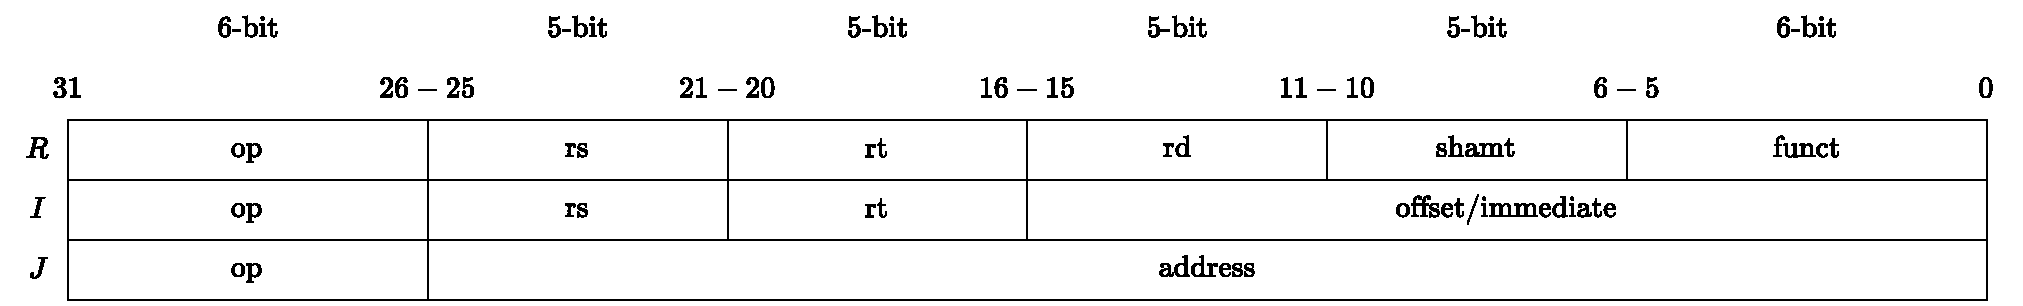
\includegraphics[width=\textwidth]{img/mips-arch.pdf}
    \caption{MIPS 32-bit architecture.}
\end{figure}

\noindent
Scan (or click) the QR code below to view the table in high quality:
\begin{center}
    \qrcode{https://github.com/AndreVale69/HPC-E-PoliMI-university-notes/tree/main/advanced-computer-architectures/notes/img/mips-arch.pdf}
\end{center}

\newpage

\begin{center}
    \large
    \textcolor{Red3}{\textbf{Phases of execution of MIPS Instructions}}
    \index{Program Counter (PC)}
    \index{Instruction Memory (IM)}
    \index{Register File (RF)}
    \index{Data Memory (DM)}
    \label{Phases of execution of MIPS Instructions}
\end{center}
Every instruction in the MIPS subset can be implemented in \textbf{\underline{at most} 5 clock cycles (phases)} as follows:
\begin{enumerate}
    \item \definition{Instruction Fetch (IF)}
    \begin{enumerate}
        \item \textbf{Send} the \textbf{content} of Program Counter (PC) register to the Instruction Memory (IM);

        \item \textbf{Fetch} the current \textbf{instruction} from Instruction Memory;
        
        \item \textbf{Update} the Program Counter to the \textbf{next sequential address} by adding the value 4 to the Program Counter (4 because each instruction is 4 bytes!).
    \end{enumerate}
    
    \item \definition{Instruction Decode and Register Read (ID)}
    \begin{enumerate}
        \item Make the \textbf{fixed-filed recording} (\textbf{decode the current instruction});
        
        \item \textbf{Read} from the Register File (RF) of one or two registers corresponding to the registers specified in the instruction fields;
        
        \item Sign-extension of the offset field of the instruction in case it is needed.
    \end{enumerate}

    \item \definition{Execution (EX)}. The ALU operates on the operands prepared in the previous cycle depending on the instruction type (see more details after this list):
    \begin{itemize}
        \item \textbf{Register-Register} ALU instructions: ALU \textbf{executes the specified operation} on the operands read from the Register File.

        \item \textbf{Register-Immediate} (Register-Constant) ALU instructions: ALU executes the specified operation on the first operand read from Register File and the sign-extended immediate operand.

        \item \textbf{Memory Reference}: ALU adds the base register and the offset to calculate the \textbf{effective address}.

        \item \textbf{Conditional Branches}: ALU compares the two registers read from Register File and computes the possible \textbf{branch target address} by adding the sign-extended offset to the incremented Program Counter.
    \end{itemize}

    \item \definition{Memory Access (ME)}. It depends on the operation performed:
    \begin{itemize}
        \item \underline{\textbf{Load}}. Instructions require a \textbf{read access to the Data Memory using the effective address}.

        \item \underline{\textbf{Store}}. Instruction require a \textbf{write access to the Data Memory using the effective address} to write the data \textbf{from the source register read from the Register File}.

        \item \underline{\textbf{Conditional branches}} can \textbf{update the content of the Program Counter} with the branch target address, if the conditional test yielded true.
    \end{itemize}

    \newpage

    \item \definition{Write-Back (WB)}. It depends on the operation performed:
    \begin{enumerate}
        \item \underline{\textbf{Load}} instructions \textbf{write the data read from memory in the destination register of the Register File}.

        \item \underline{\textbf{ALU}} instructions \textbf{write the ALU results into the destination register of the Register File}.
    \end{enumerate}
\end{enumerate}

\begin{flushleft}
    \textcolor{Red3}{\textbf{Execution (EX) details}}\label{Execution (EX) details}
\end{flushleft}
\begin{itemize}
    \item \textbf{Register-Register ALU instructions}. Given the following pattern (where \texttt{op} can be the operators \texttt{add/addi} (+) or \texttt{sub/subi} (-), but not \texttt{mult} ($\times$) or \texttt{div} ($\div$) because they required some special registers and therefore more phases):
    \lstinputlisting[language=misc]{code/mips-architecture/alu-instructions-1.s}
    \textbf{Cost: 4 clock cycles}
    \begin{enumerate}
        \item Instruction Fetch (IF) and update the Program Counter (next sequential address);

        \item Fixed-Field Decoding and read from Register File the registers: \texttt{y} and \texttt{z};
        
        \item Execution (EX), ALU performs the operation \texttt{op} (\texttt{\$ y op \$ z});

        \item Write-Back (WB), ALU writes the result into the destination register \texttt{x}.
    \end{enumerate}

    \item \textbf{Memory Reference}
    \begin{itemize}
        \item \underline{Load}. Given the following pattern:
        \lstinputlisting[language=misc]{code/mips-architecture/alu-instructions-2.s}
        \textbf{Cost: 5 clock cycles}
        \begin{enumerate}
            \item Instruction Fetch (IF) and update the Program Counter (next sequential address);

            \item Fixed-Field Decoding and read of Base and register \texttt{y} from Register File (RF);

            \item Execution (EX), ALU adds the base register and the offset to calculate the effective address: \texttt{y + offset};

            \item Memory Access (ME), read access to the Data Memory (DM) using the effective (\texttt{y + offset}) address;

            \item Write-Back (WB), write the data read from memory in the destination register of the Register File (RF) \texttt{x}.
        \end{enumerate}

        \newpage

        \item \underline{Store}. Given the following pattern:
        \lstinputlisting[language=misc]{code/mips-architecture/alu-instructions-3.s}
        \textbf{Cost: 4 clock cycles}
        \begin{enumerate}
            \item Instruction Fetch (IF) and update the Program Counter (next sequential address);

            \item Fixed-Field Decoding and read of Base register \texttt{y} and source register \texttt{x} from Register File (RF);

            \item Execution (EX), ALU adds the base register and the offset to calculate the effective address: \texttt{y + offset};

            \item Memory Access (WB), write the data read from memory in the destination register of the Register File (RF) \texttt{M(y + offset)}.
        \end{enumerate}
    \end{itemize}

    \item \textbf{Conditional Branch}. Given the following pattern:
    \lstinputlisting[language=misc]{code/mips-architecture/alu-instructions-4.s}
        \textbf{Cost: 4 clock cycles}
        \begin{enumerate}
            \item Instruction Fetch (IF) and update the Program Counter (next sequential address);

            \item Fixed-Field Decoding and read of source registers \texttt{x} and \texttt{y} from Register File (RF);

            \item Execution (EX), ALU compares two registers \texttt{x} and \texttt{y} and compute the possible branch target address by adding the sign-extended offset to the incremented Program Counter: \texttt{PC + 4 + offset};

            \item Memory Access (ME), update the content of the Program Counter with the branch target address (we assume that the conditional test is true).
        \end{enumerate}
\end{itemize}
    \subsubsection{Implementation of MIPS processor - Data Path}

Implementing a MIPS processor isn't difficult. On the following page we show three different diagrams: the first is a very high level data path to allow the reader to understand how it works; the second is more detailed, but without the CU (Control Unit); the third is the complete data path and it also includes the CU (in red).

\begin{figure}[!htp]
    \centering
    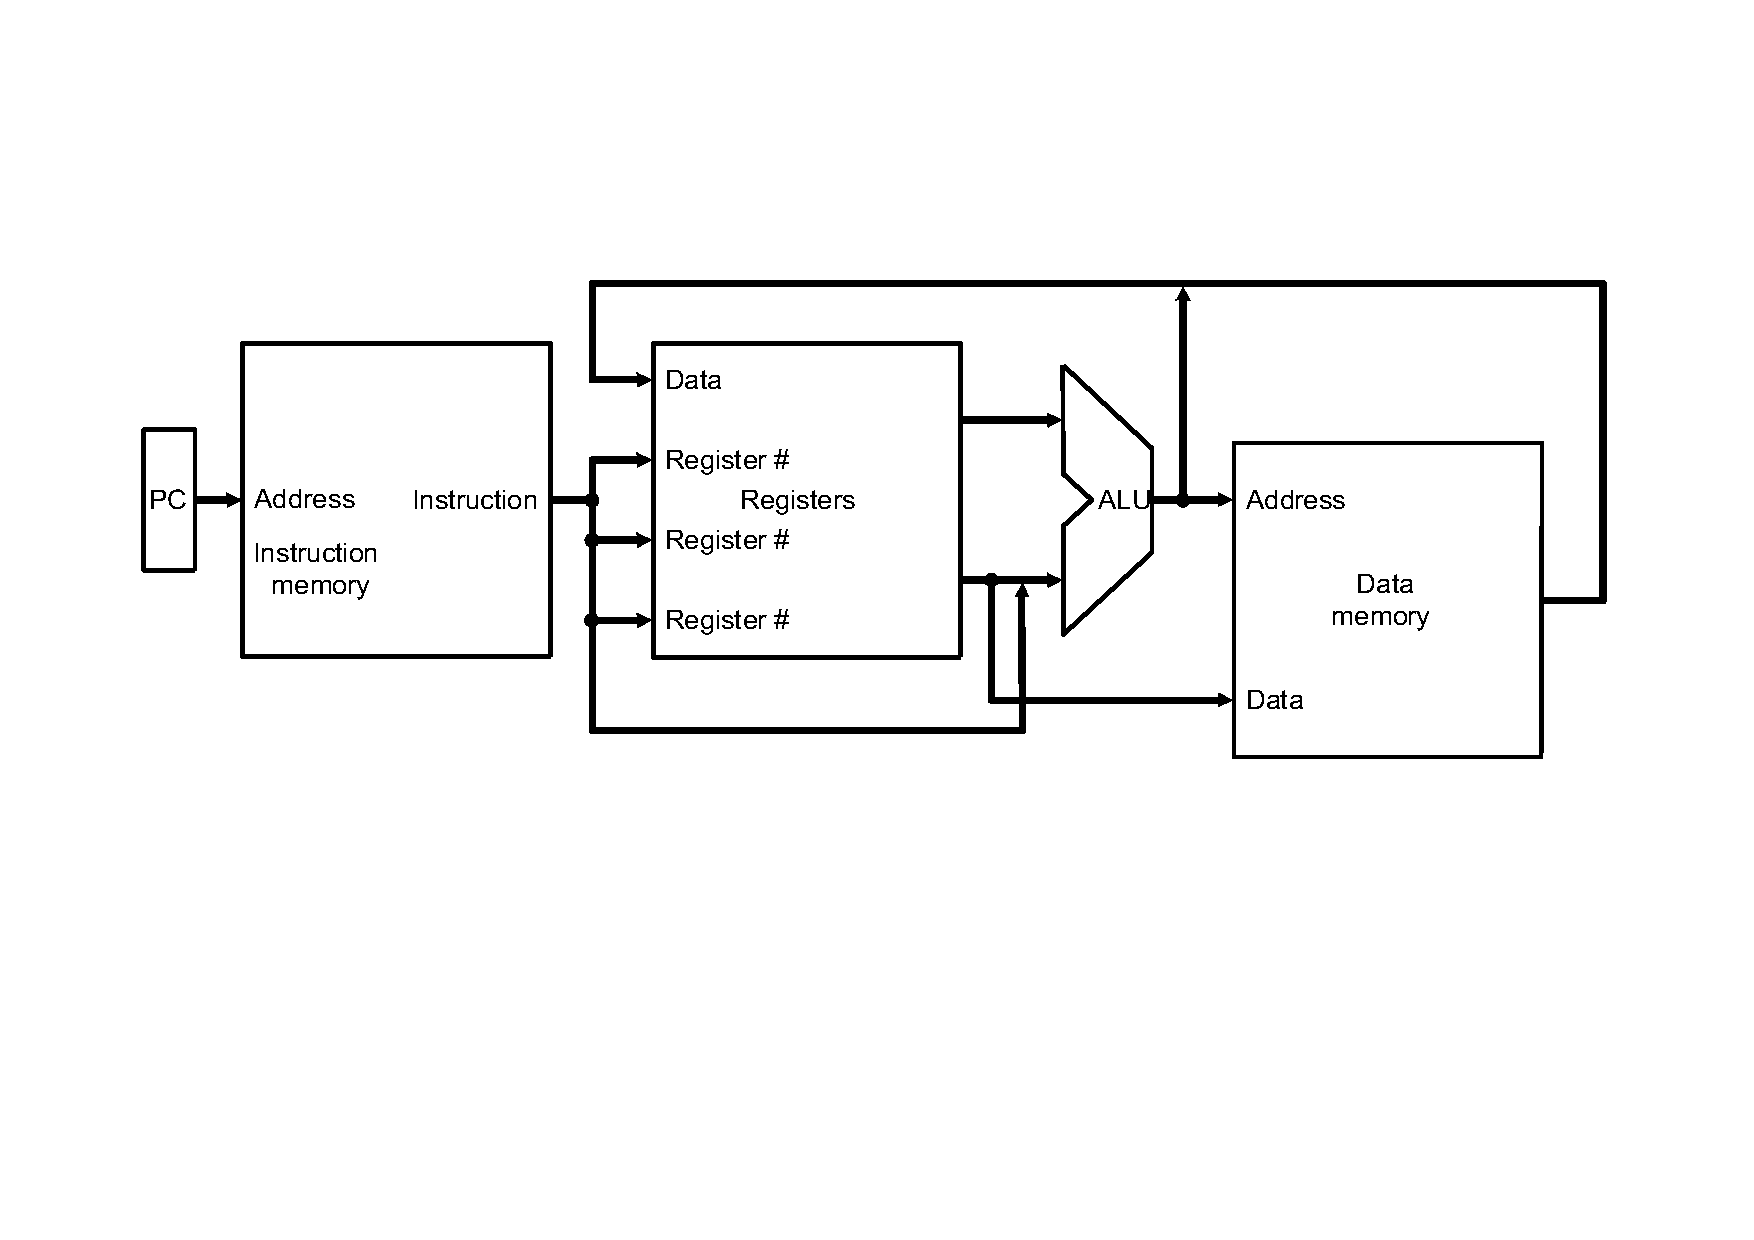
\includegraphics[width=\textwidth]{img/basic-implementation-mips-datapath.pdf}
    \caption{A basic implementation of MIPS data path.\cite{pipelining-slides}}
    \label{fig: basic implementation of MIPS data path}
\end{figure}

\noindent
Scan (or click) the QR code below to view the figure~\ref{fig: basic implementation of MIPS data path} in high quality:
\begin{center}
    \qrcode{https://github.com/PoliMI-HPC-E-notes-projects-AndreVale69/HPC-E-PoliMI-university-notes/tree/main/advanced-computer-architectures/notes/img/basic-implementation-mips-datapath.pdf}
\end{center}
Two notes:
\begin{itemize}
    \item The \textbf{Instruction Memory} (read-only memory) is separated from \textbf{Data Memory}.
    
    \item The 32 general-purpose register are organized in a \textbf{Register File} (RF) with 2 read ports and 1 write port.
\end{itemize}

\begin{figure}[!htp]
    \centering
    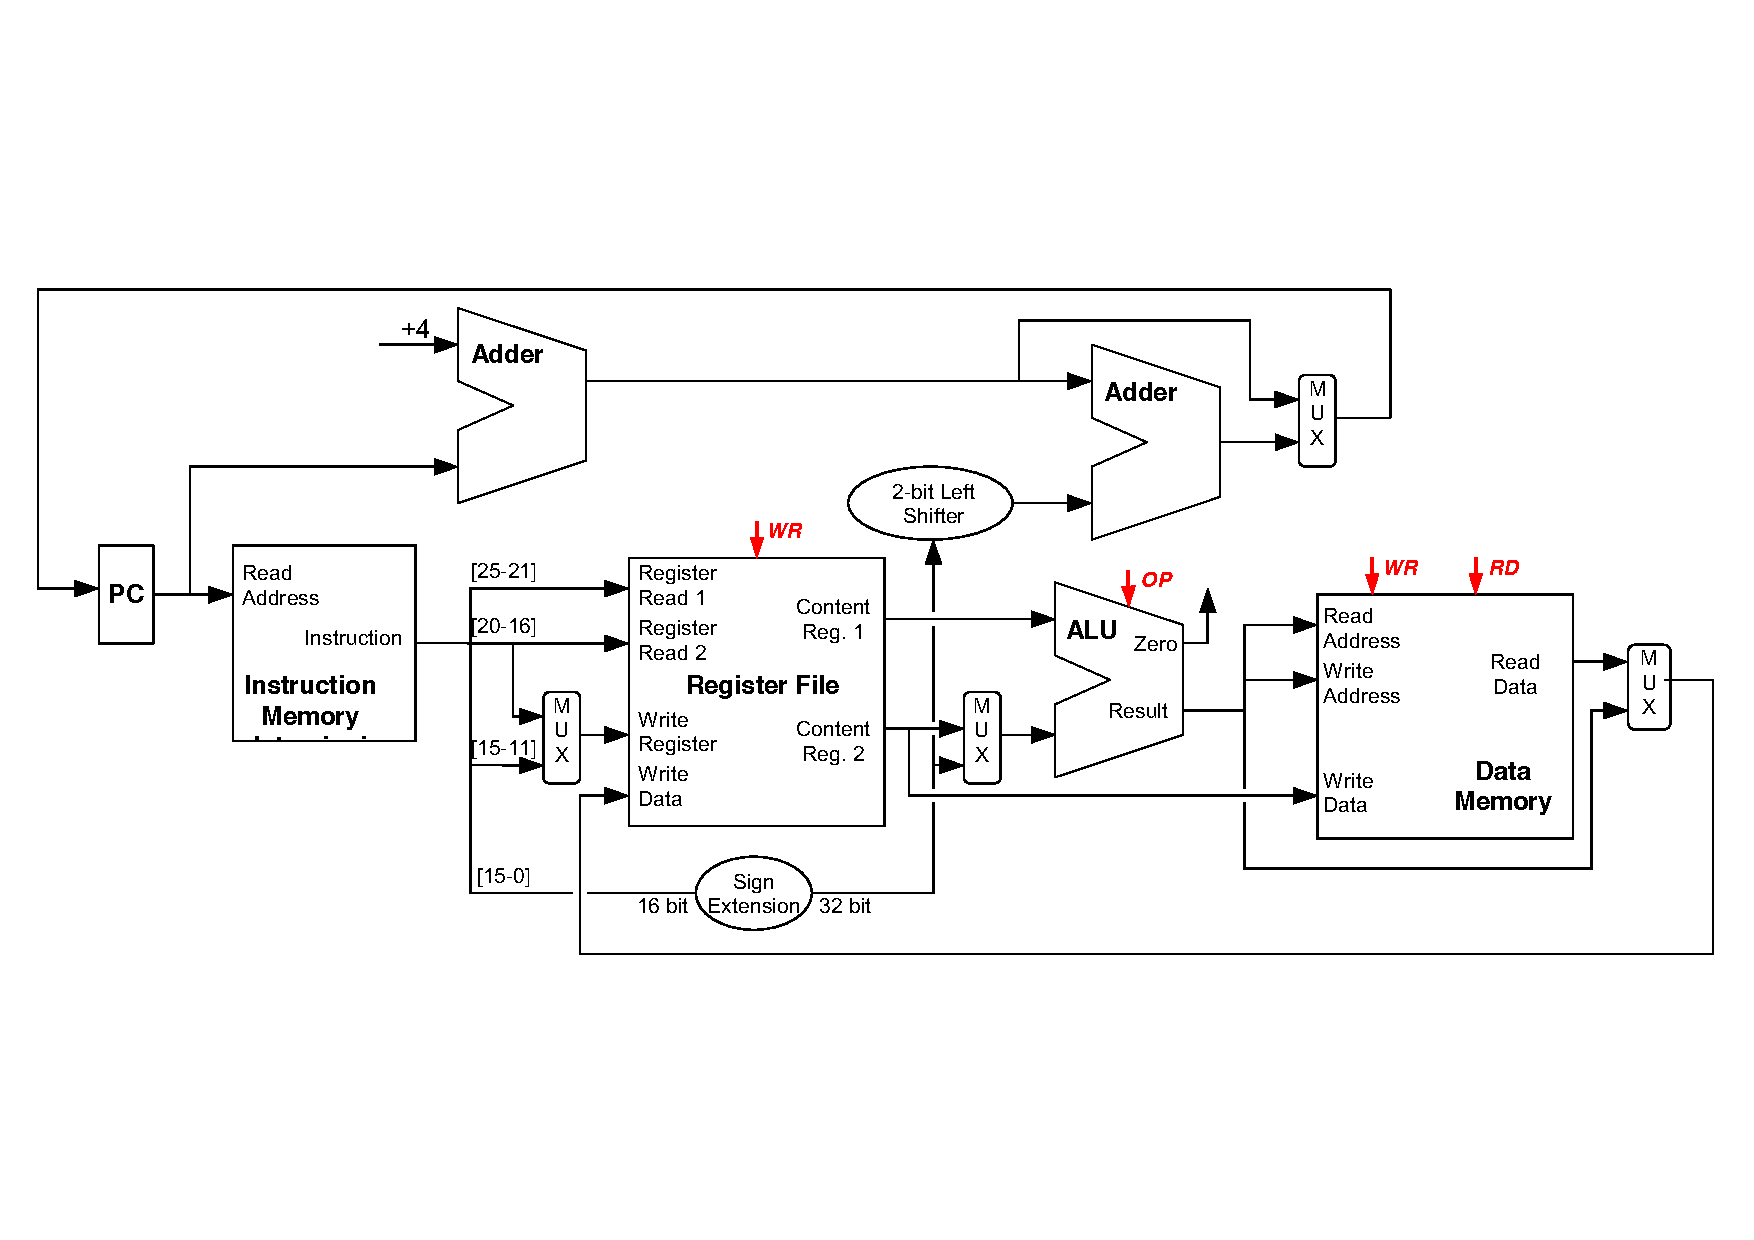
\includegraphics[width=\textwidth]{img/implementation-mips-datapath.pdf}
    \caption{An implementation of MIPS data path (no Control Unit).\cite{pipelining-slides}}
    \label{fig: implementation of MIPS data path (no Control Unit)}
\end{figure}

\newpage

\noindent
Scan (or click) the QR code below to view the figure~\ref{fig: implementation of MIPS data path (no Control Unit)} in high quality:
\begin{center}
    \qrcode{https://github.com/PoliMI-HPC-E-notes-projects-AndreVale69/HPC-E-PoliMI-university-notes/tree/main/advanced-computer-architectures/notes/img/implementation-mips-datapath.pdf}
\end{center}

\begin{figure}[!htp]
    \centering
    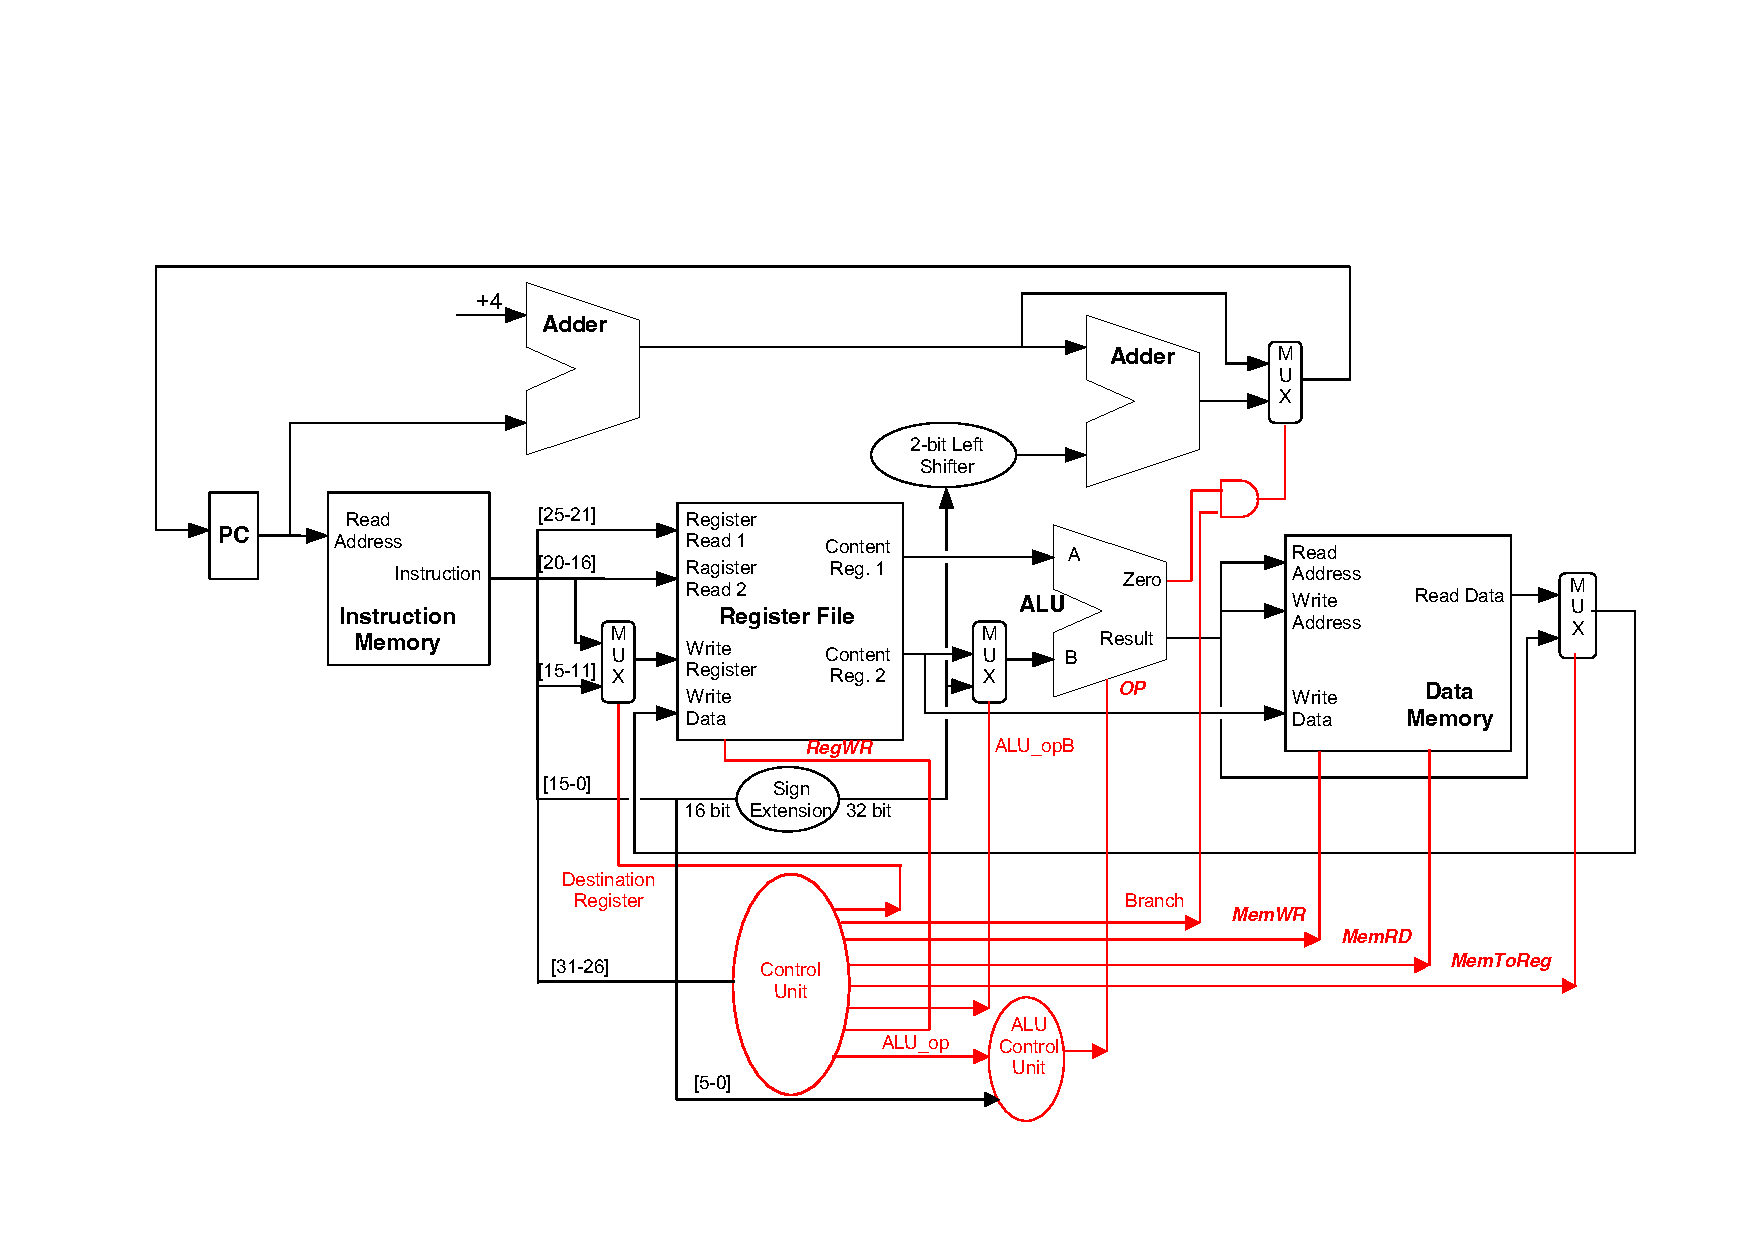
\includegraphics[width=\textwidth]{img/implementation-mips-datapath-cu.pdf}
    \caption{A complete implementation of MIPS data path.\cite{pipelining-slides}}
    \label{fig: complete implementation of MIPS data path}
\end{figure}

\noindent
Scan (or click) the QR code below to view the figure~\ref{fig: complete implementation of MIPS data path} in high quality:
\begin{center}
    \qrcode{https://github.com/PoliMI-HPC-E-notes-projects-AndreVale69/HPC-E-PoliMI-university-notes/tree/main/advanced-computer-architectures/notes/img/implementation-mips-datapath-cu.pdf}
\end{center}
    \subsubsection{MIPS Pipelining}

In simple words, the Instruction Pipelining (or Pipelining) is a technique for implementing instruction-level parallelism within a single processor. Pipelining attempts to keep every part of the processor busy with some instruction by dividing incoming instructions into a series of sequential steps (the eponymous \dquotes{pipeline}) performed by different processor units with different parts of instructions processed in parallel.

\highspace
\begin{definitionbox}
    \definition{Pipelining} is a performance optimization technique based on the \textbf{overlap} of the execution of multiple instructions deriving from a sequential execution flow.
\end{definitionbox}

\noindent
Pipelining exploits the \textbf{parallelism among instructions in a sequential instruction stream}.

\begin{flushleft}
    \textcolor{Red2}{\faIcon[regular]{star} \textbf{Basic idea}}
\end{flushleft}
The execution of an \textbf{instruction is divided into different phases} (called \definition{pipelines stages}), requiring a fraction of the time necessary to complete the instruction. These stages are connected one to the next to form the pipeline: 
\begin{enumerate}
    \item Instructions enter the pipeline at one end;
    \item Progress through the stages;
    \item And exit from the other end.
\end{enumerate}
As in the assembly line.

\begin{flushleft}
    \textcolor{Green3}{\faIcon{check} \textbf{Advantage}}
\end{flushleft}
The \textbf{Pipelining is transparent for the programmer}. To understand what it means, let's make an example.

\begin{examplebox}
    Image a car assembly line (e.g. Ferrari). A new car exits from the Ferrari assembly line in the time necessary to complete one of the phases. The pipelining technique doesn't reduce the time required to complete a car (the \textbf{latency}), BUT increases the number of vehicles produced per time unit (the \textbf{throughput}) and the frequency to complete cars.
\end{examplebox}

\newpage

\begin{examplebox}
    Image a sequential laundry jobs over time:\cite{pipelining-slides}
    \begin{center}
        \centering
        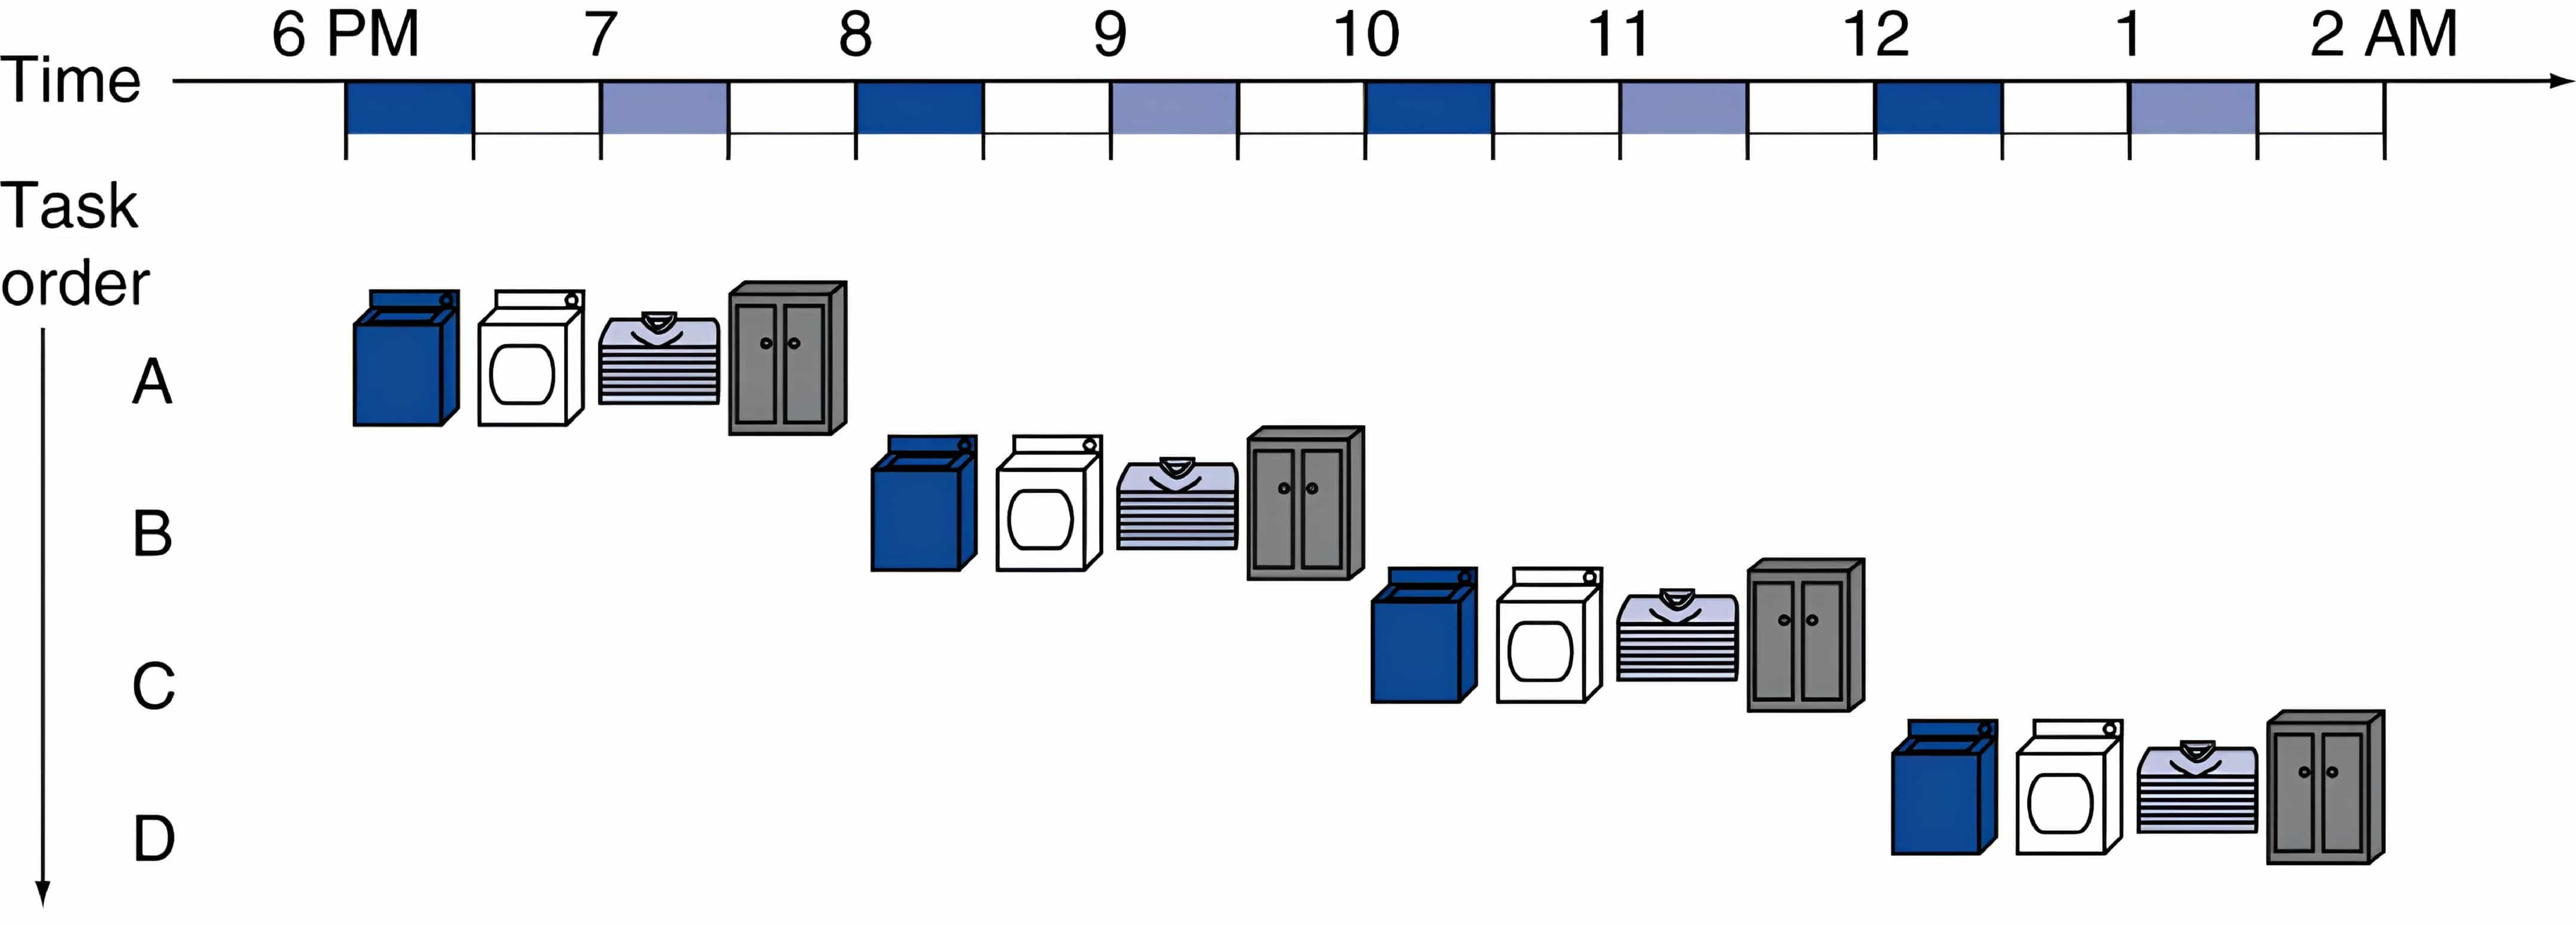
\includegraphics[width=.9\textwidth]{img/pipelining-example-1.pdf}
    \end{center}
    The pipelined laundry. Overlapping execution of stages to improve throughput (number of jobs executed per hour):\cite{pipelining-slides}
    \begin{center}
        \centering
        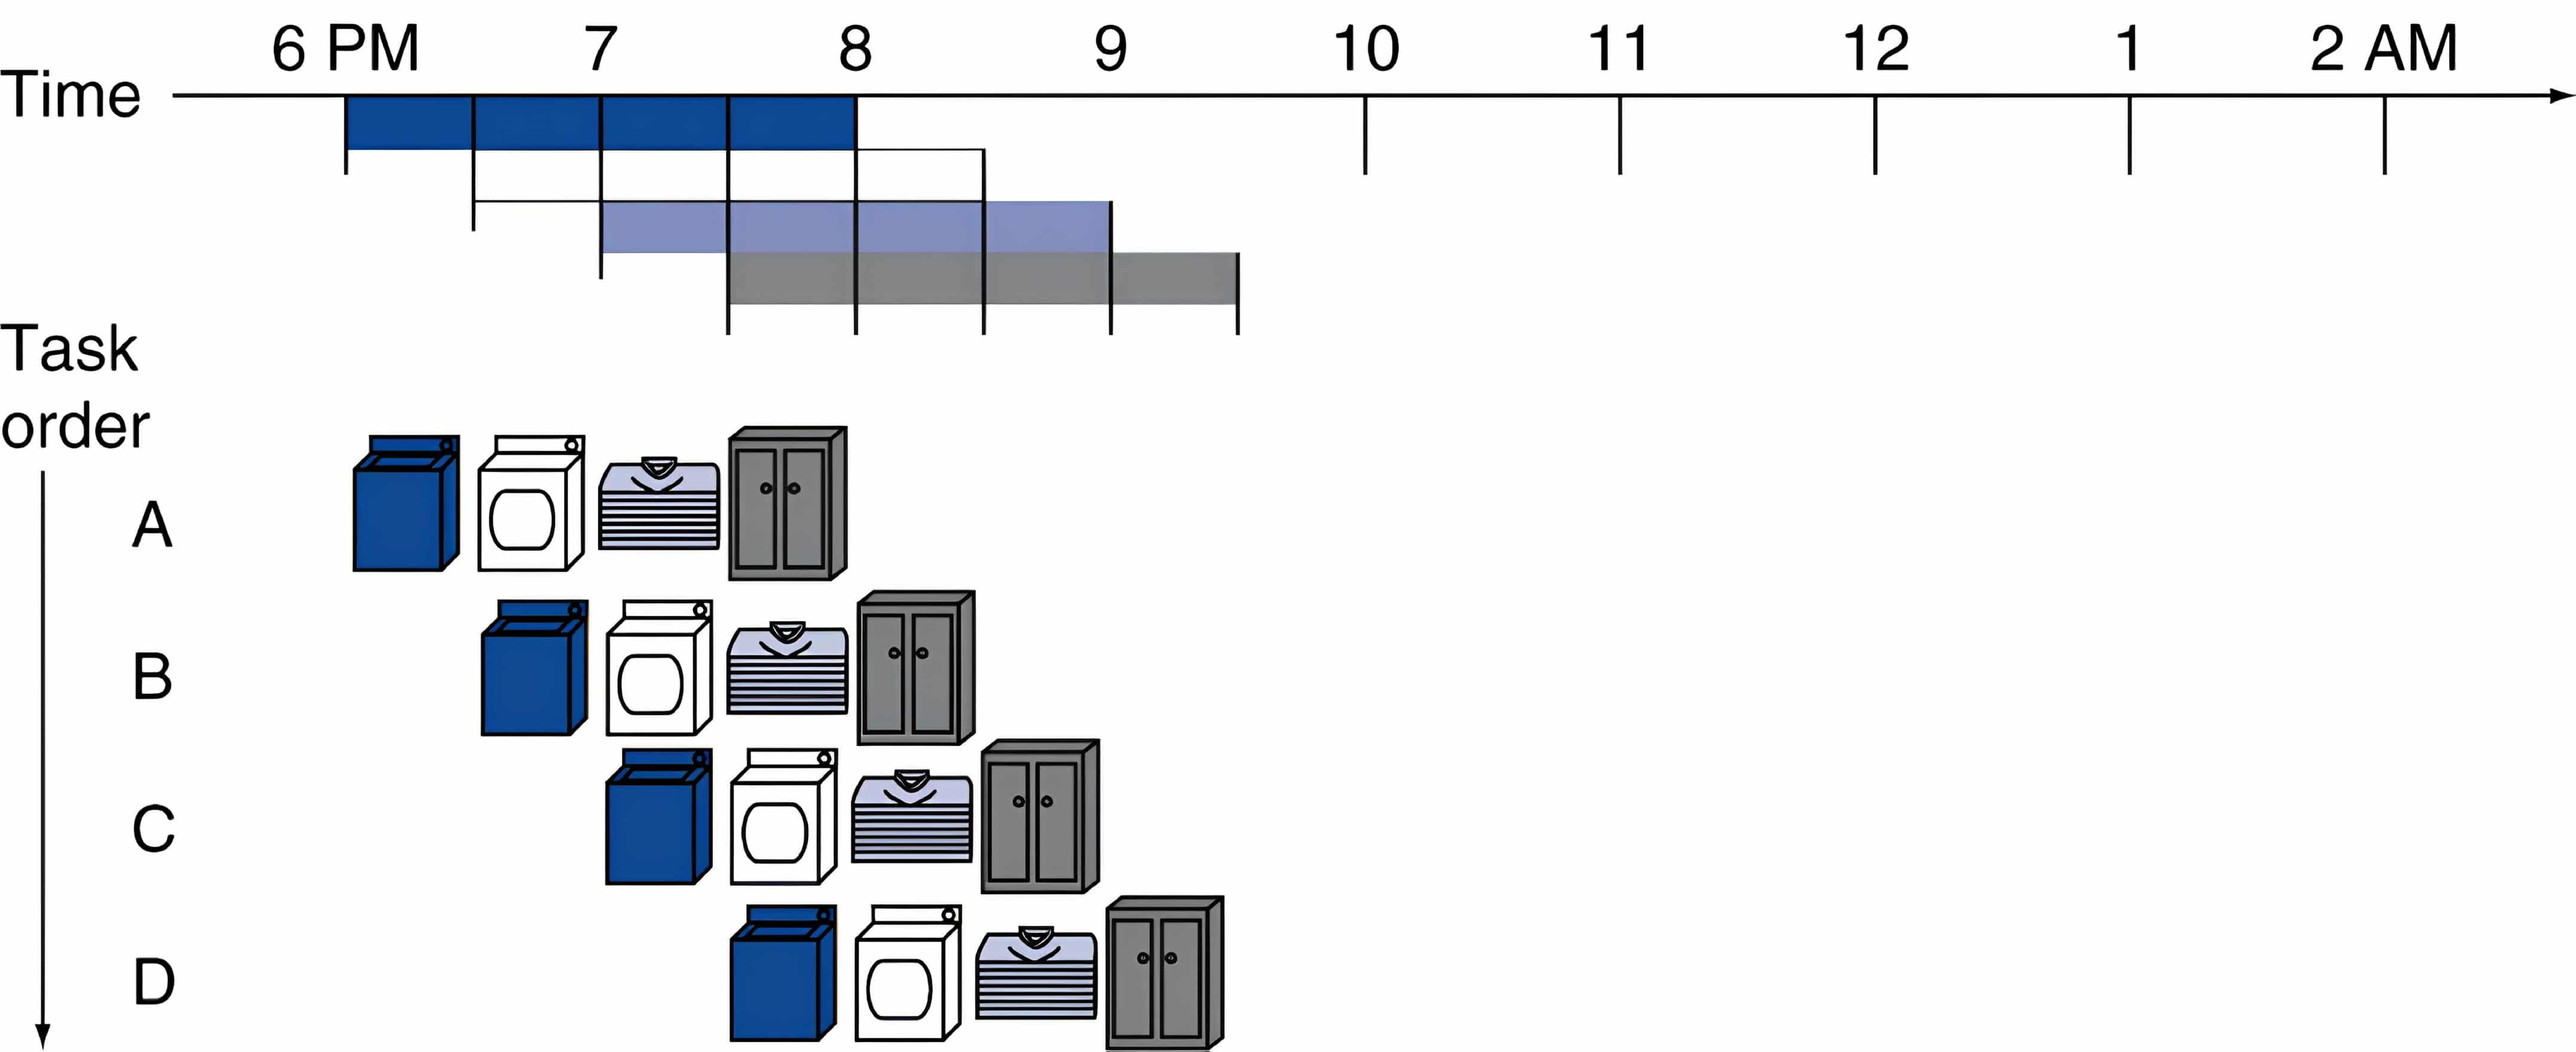
\includegraphics[width=.9\textwidth]{img/pipelining-example-2.pdf}
    \end{center}
\end{examplebox}

\noindent
As introduced in the previous example, sequential execution is slower than pipelining. The following figure shows the difference (in terms of clock cycles) between sequential and pipelining.
\begin{figure}[!htp]
    \centering
    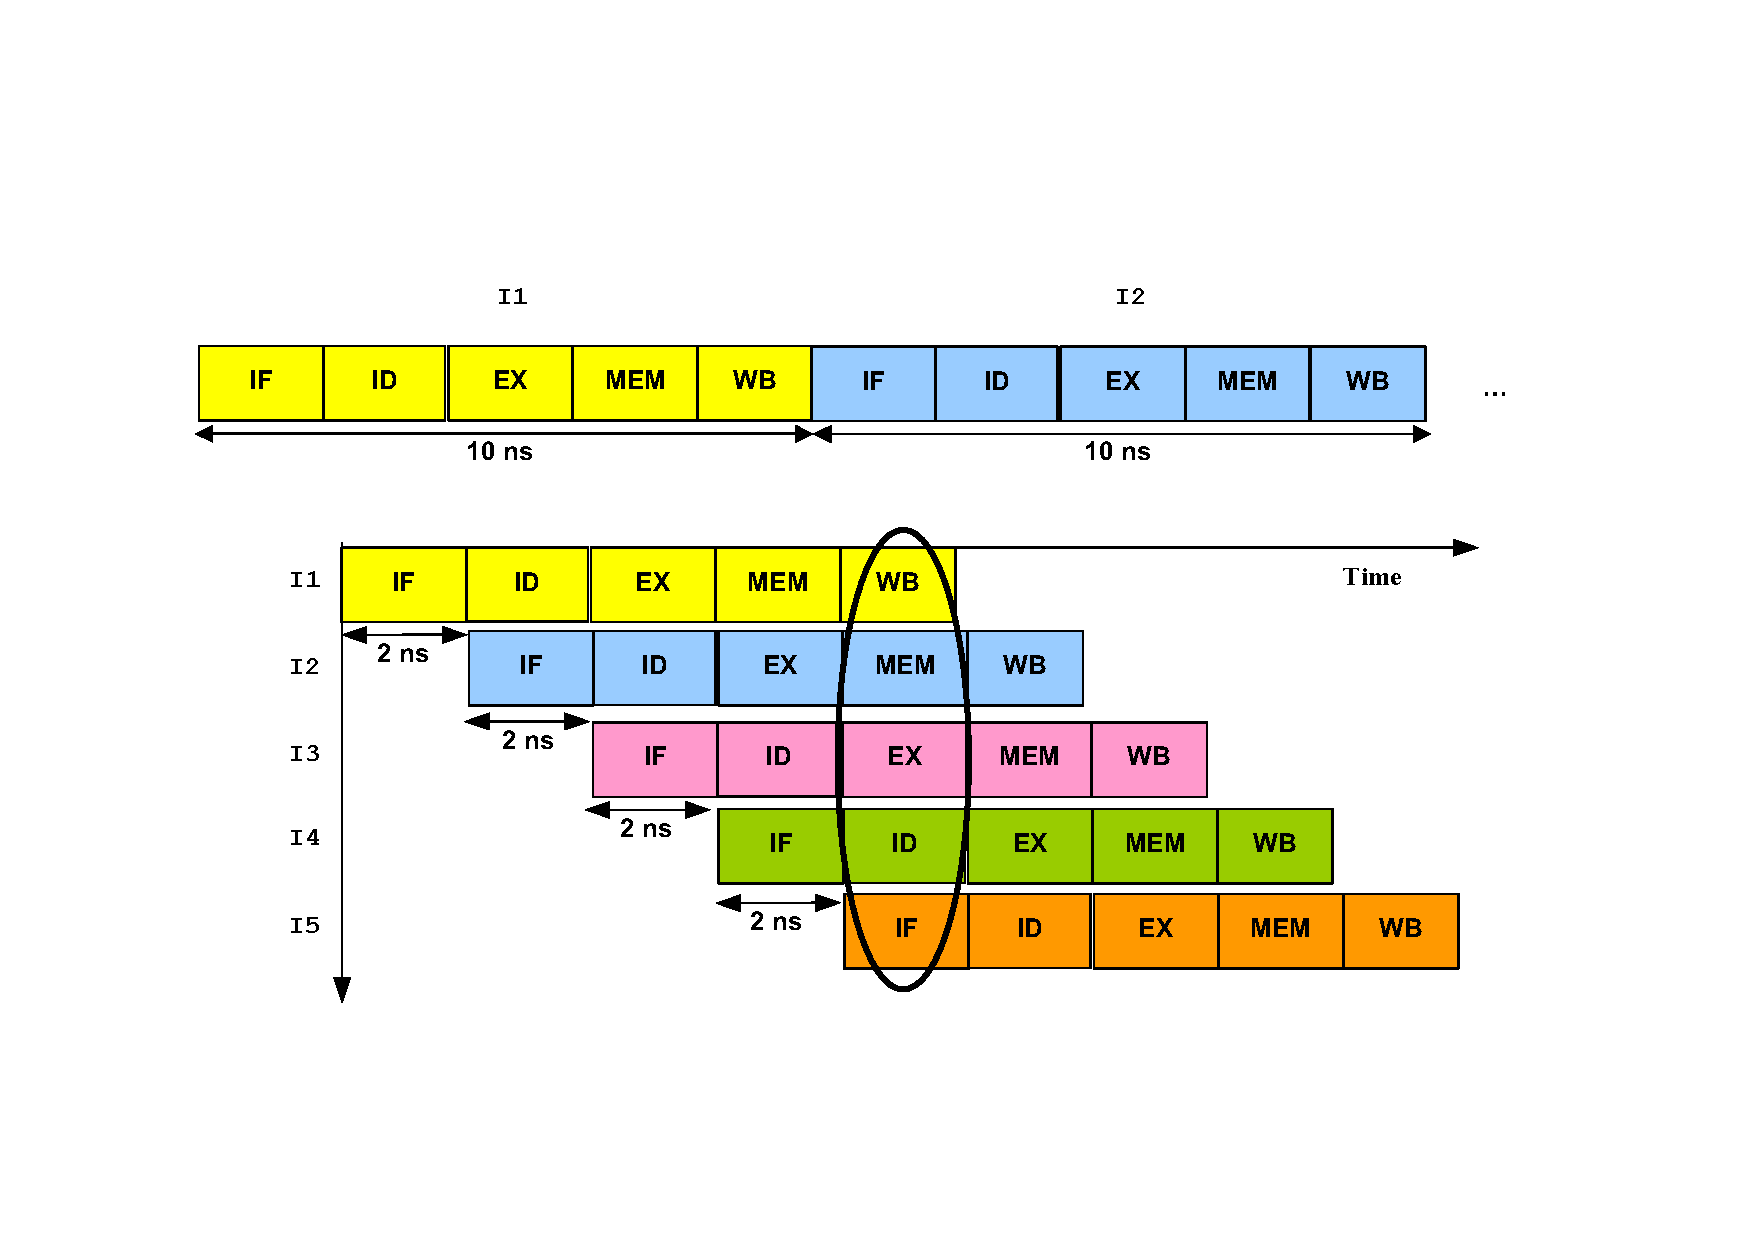
\includegraphics[width=\textwidth]{img/sequential-vs-pipelining-1.pdf}
    \caption{Sequential vs Pipelining.\cite{pipelining-slides}}
    \label{fig: sequential vs pipelining}
\end{figure}

\newpage

\noindent
The time to advance the instruction of one stage in the pipeline corresponds to a clock cycle. So the total cost is: 9 clock cycles.

\highspace
It's obvious that the \textbf{pipeline stages must be synchronized}: the duration of a clock cycle is defined by the time required by the slower stage in the pipeline (i.e. 2 ns). The \textbf{main goal} is to \textbf{balance the length of each pipeline stage}. If the stages are perfectly balanced, the \textbf{ideal speedup} due to pipelining is equal to the number of pipeline stages.

\begin{definitionbox}
    The \definition{ideal speedup} must be the \textbf{same value of the pipeline stages}.
\end{definitionbox}

\highspace
Look again at Figure~\ref{fig: sequential vs pipelining}. The sequential and pipelining cases consist of 5 instructions, each of which is divided into 5 low-level instructions of 2 ns each.
\begin{itemize}
    \item The \textbf{latency} (total execution time) of each instruction is not varied, it's always 10 ns.
    \begin{definitionbox}
        The \definition{latency} is the execution time of a single instruction.
    \end{definitionbox}

    \item The \textbf{throughput} (number of low-level instructions completed in the time unit) is improved:
    \begin{itemize}
        \item Sequential: 5 instructions in 50 ns (1 instruction per 10 ns, $50 \div 5 = 10$)
        \item Pipelining: 5 instruction in 18 ns (1 instruction per 3.6 ns, $18 \div 5 = 3.6$)
    \end{itemize}
    \begin{definitionbox}
        The \definition{throughput} is the number of instructions completed per unit of time.
    \end{definitionbox}
\end{itemize}

\newpage

\begin{center}
    \large
    \textcolor{Red3}{\textbf{Pipeline Execution of MIPS Instructions}}
\end{center}
On page~\pageref{Execution (EX) details} we discussed some MIPS instructions to understand how the MIPS architecture works. The aim of the following pages is to understand \textbf{how MIPS works in a pipelined execution}.

\highspace
We want to perform the following assembly lines:
\lstinputlisting[language=misc]{code/mips-pipelining/sequential-vs-pipelining.s}
\begin{figure}[!htp]
    \centering
    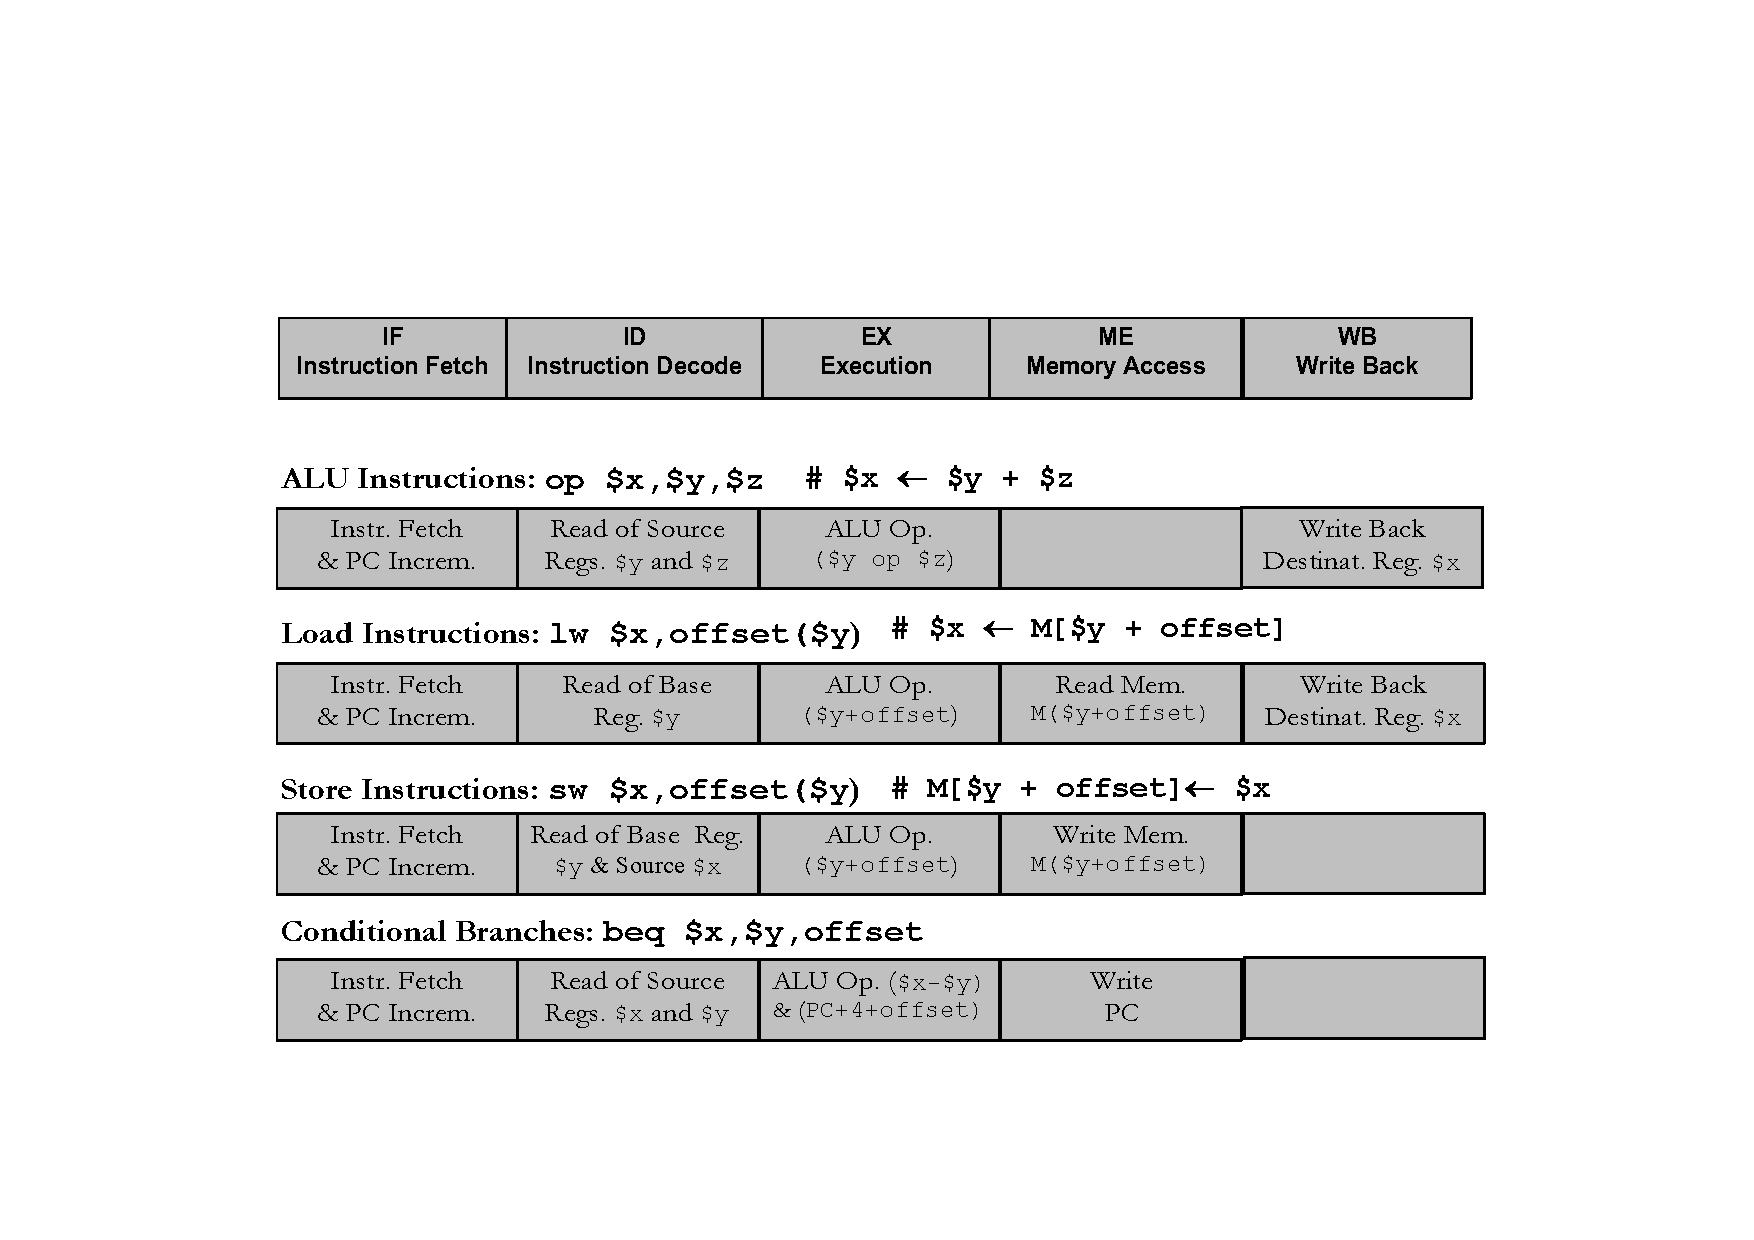
\includegraphics[width=\textwidth]{img/sequential-vs-pipelining-2.pdf}
    \caption{Pipeline Execution of MIPS Instructions.\cite{pipelining-slides}}
\end{figure}

\newpage

\begin{center}
    \textcolor{Red3}{\textbf{Resources used during the pipeline execution}}
\end{center}
\begin{figure}[!htp]
    \centering
    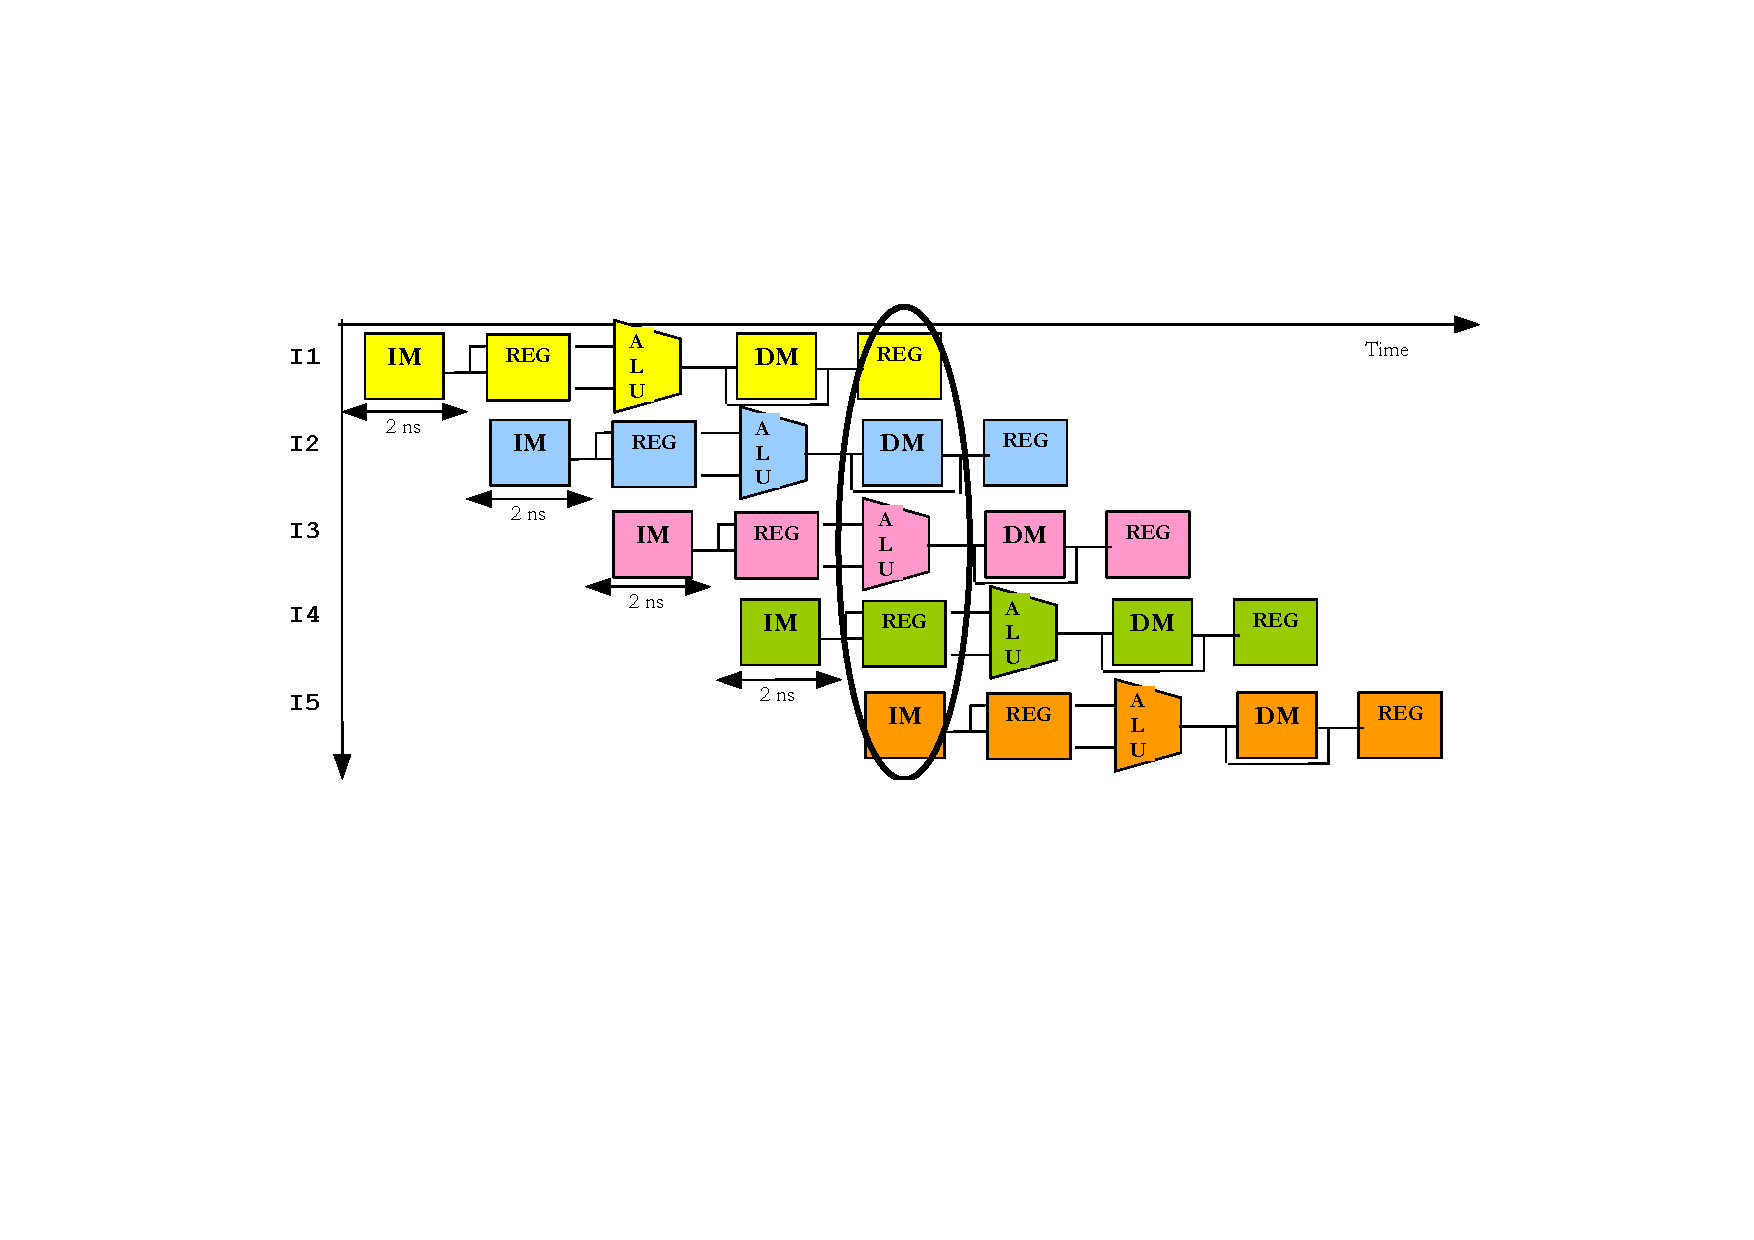
\includegraphics[width=\textwidth]{img/sequential-vs-pipelining-3.pdf}
    \caption{Resources used during the pipeline execution (IM is Instruction Memory, REG is Register File and DM is Data Memory).\cite{pipelining-slides}}
\end{figure}

\newpage

\begin{center}
    \large
    \textcolor{Red3}{\textbf{Implementation of MIPS pipeline}}
\end{center}
The division of the execution of each instruction in $n$ stages implies that in each clock cycle, there are $n$ instructions for execution. That means the CPU must have $n$ modules corresponding to $n$ execution stages. Therefore, to do pipelining, we need \definition{pipeline registers} \textbf{to separate the different stages}.

\highspace
In the following figure, we can see how the pipeline registers are implemented. Between each phase of execution of MIPS instructions (details on page \pageref{Phases of execution of MIPS Instructions}), there is a pipeline register holding the result of the instruction.
\begin{figure}[!htp]
    \centering
    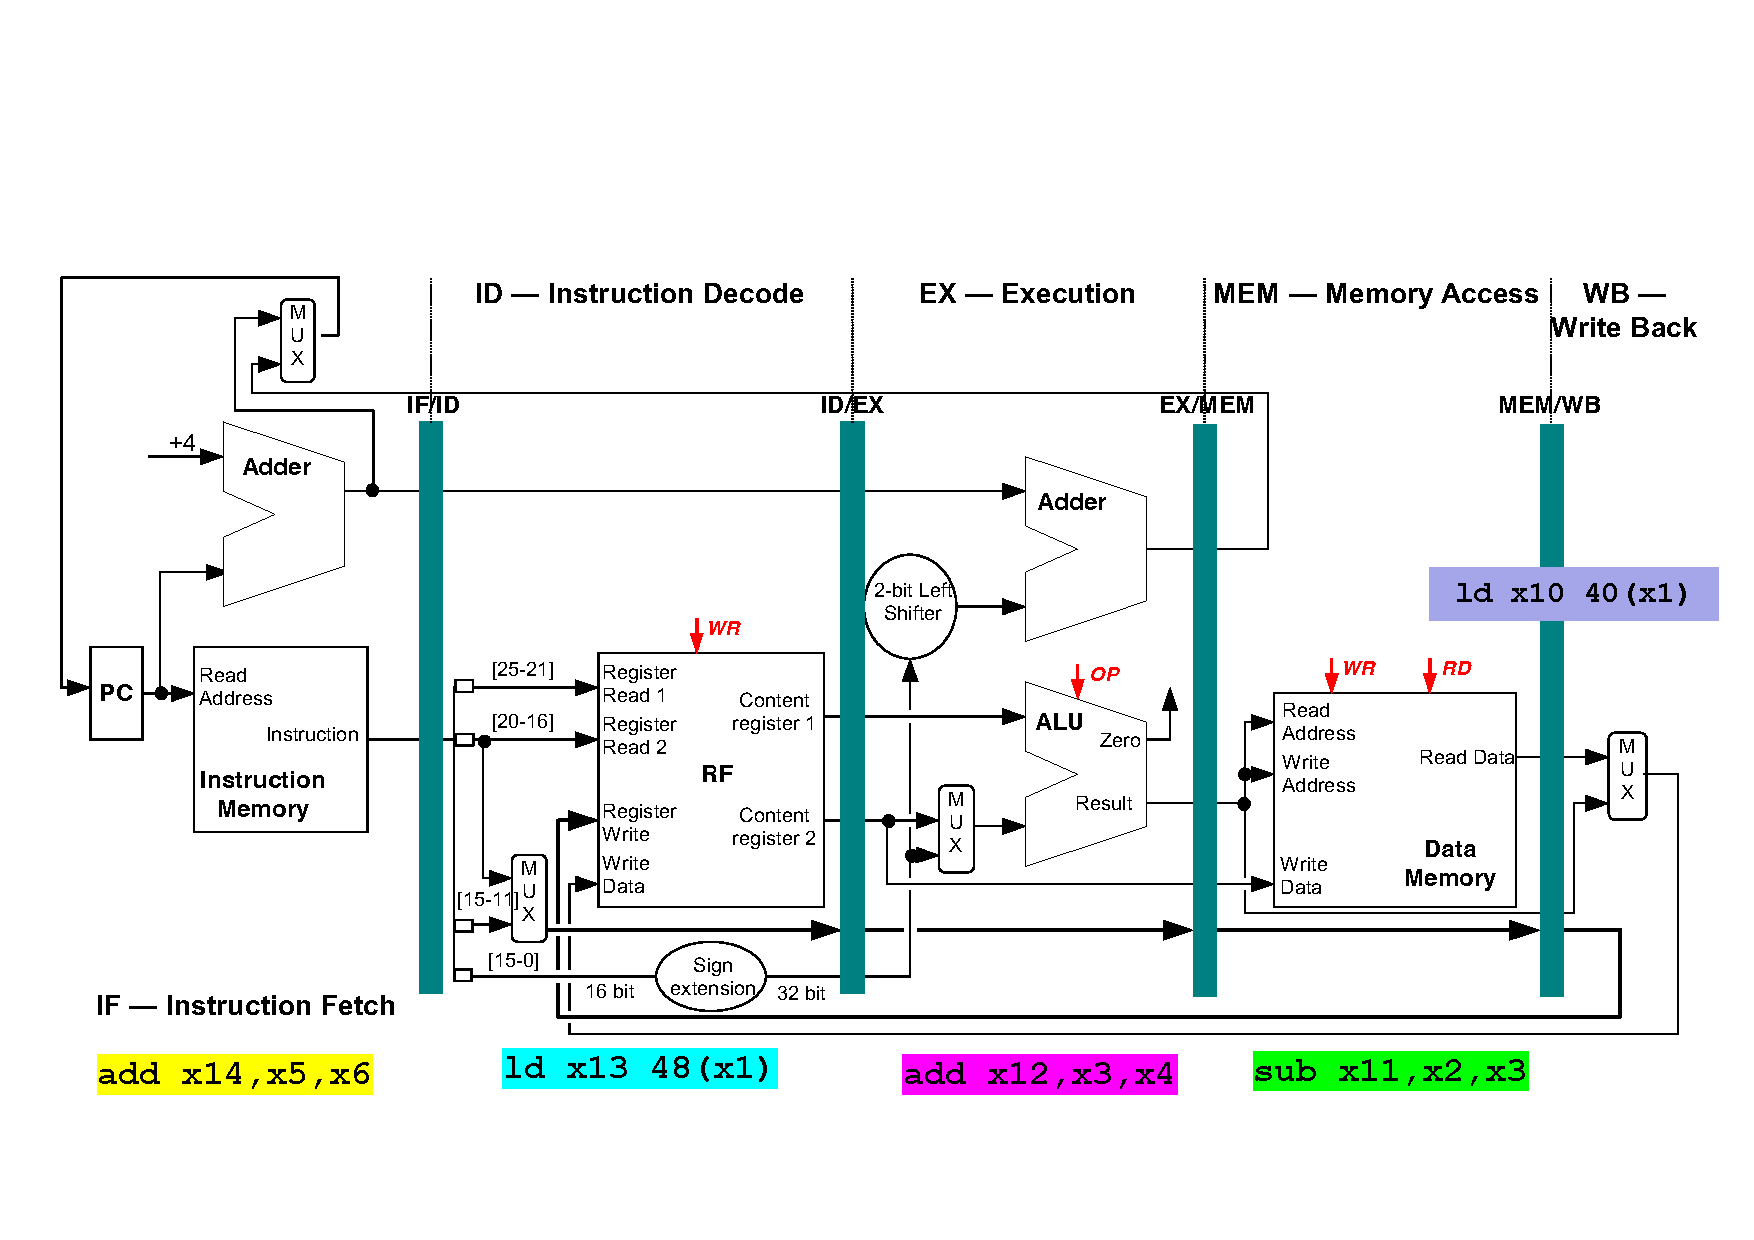
\includegraphics[width=\textwidth]{img/pipeline-registers-1.pdf}
    \caption{MIPS pipeline implementation.\cite{pipelining-slides}}
\end{figure}

\noindent
\underline{Note}: \textbf{the data stored in the interstage registers correspond (obviously) to different instructions}.

\newpage

\noindent
Finally, in the following figure we can see the timeline implementation of the pipeline registers. But there are two basic assumptions to make:
\begin{enumerate}
    \item There are no data dependencies between instructions. If there were, an instruction could read a register with an unknown value (Pipeline Hazard, page~\pageref{subsubsection: The problem of Pipeline Hazards}).

    \item There are no branch/jump instructions.
\end{enumerate}
\begin{figure}[!htp]
    \centering
    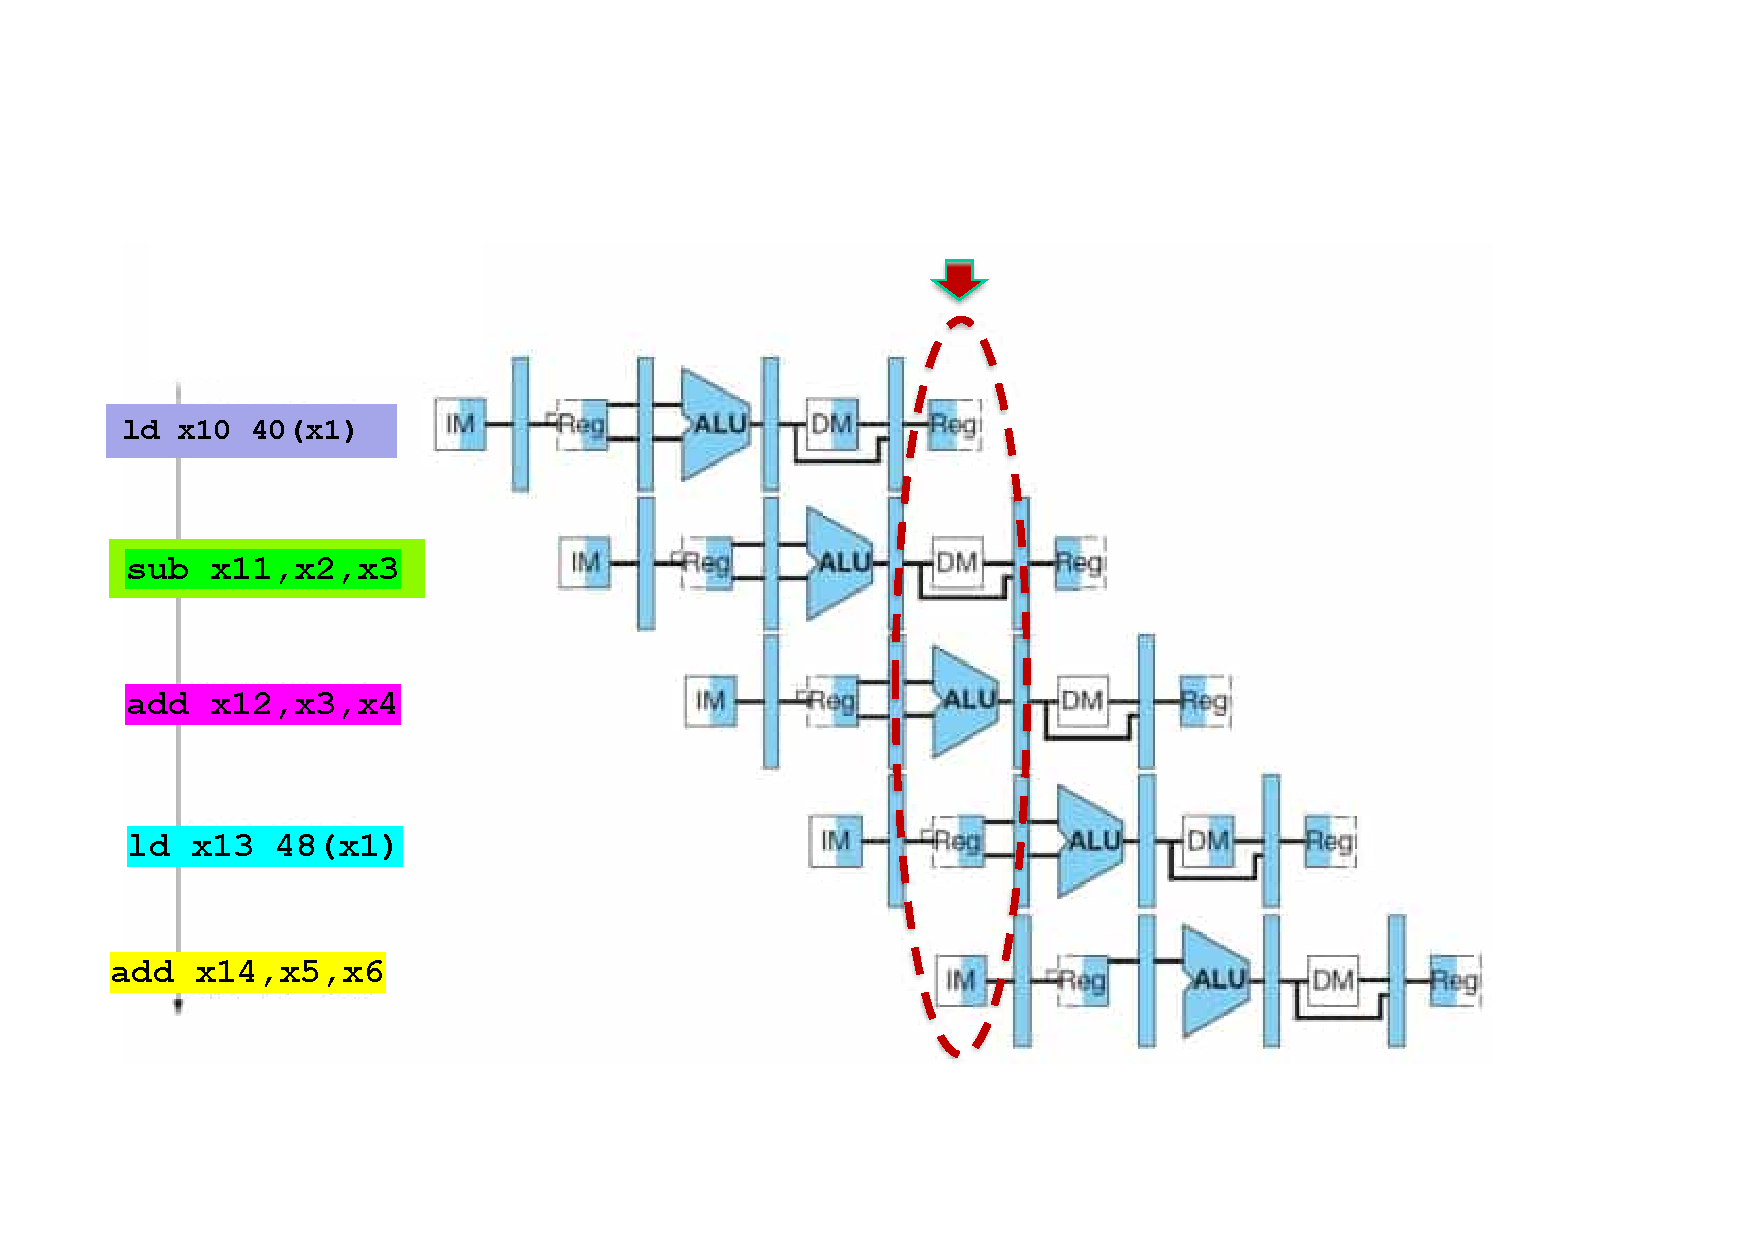
\includegraphics[width=\textwidth]{img/pipeline-registers-2.pdf}
    \caption{Timeline of MIPS pipeline implementation.\cite{pipelining-slides}}
\end{figure}
    \subsubsection{The problem of Pipeline Hazards}\label{subsubsection: The problem of Pipeline Hazards}

\begin{definitionbox}[: Hazard]
    A \definition{hazard (conflict)} is created whenever there a \textbf{dependence} between two instructions, and instructions are close enough that the overlap caused by pipelining would change the order of access to the operands involved in the dependence.
\end{definitionbox}

\begin{flushleft}
    \textcolor{Red2}{\faIcon{exclamation-triangle} \textbf{Problem Consequences}}
\end{flushleft}
The Hazards:
\begin{itemize}
    \item \textbf{Force} the next \textbf{instruction} in the pipeline \textbf{to be executed later} than its intended clock cycle.

    \item \textbf{Reduced the performance} from the ideal speedup achieved by pipelining (direct previous consequence).
\end{itemize}
There are \textbf{three classes} of Hazards:
\begin{itemize}
    \item \definition{Structural Hazards}. Attempt to use the \textbf{same resource from different instructions simultaneously}.
    
    \example{Example}: single memory for instruction and data.
    

    \item \definition{Data Hazards}. Attempt to \textbf{use a result before it is ready}.
    
    \example{Example}: instruction depending on a result of a previous instruction still in the pipeline.

    There are also \textbf{two specific forms} of data hazard, called \definition{Load-Use Data Hazard} and \definition{Load-Store Data Hazard}. Both occur when the \textbf{data loaded by a load instruction is not yet available when it is needed by another instruction}. In the case of Load-Use, the \dquotes{another instruction} is an operator such as \texttt{add}; in the case of Load-Store, the \dquotes{another instruction} is the store (\texttt{sw}) instruction.

    The following \example{example} shows the conflict (Load-Use Data Hazard) between two instructions. In particular, the value \texttt{lw} writes to \texttt{s2} is not available until \texttt{lw} has completed the \texttt{MEM} phase, but \texttt{and} needs this value when it enters the \texttt{EX} phase, i.e. when \texttt{lw} enters the \texttt{MEM} phase.
    \lstinputlisting[language=misc]{code/the-problem-of-pipeline-hazards/load-use-data-hazard.s}

    \item \definition{Control Hazards}. Attempt to \textbf{make a decision on the next instruction to execute before the condition is evaluated} (more detailed analysis on page \pageref{flushleft: how to detect Control Hazards}).
    
    \example{Example}: conditional branch execution.
\end{itemize}

\begin{flushleft}
    Structural Hazards? No problem for MIPS Architecture!
\end{flushleft}
\textbf{There aren't any structural hazards in MIPS architecture} because the Instruction Memory (IM) is separated from the Data Memory (DM). Also, the Register File (RF) is used in the same clock cycle (read access by an instruction and write access by another instruction).

\newpage

\begin{flushleft}
    \textcolor{Green3}{\faIcon{question-circle} \textbf{How to detect \underline{Data Hazards}? Dependency Analysis}}
\end{flushleft}
To \textbf{detect Data Hazards}, it is suggested to analyze the dependencies. If the instructions executed in the pipeline depend on each other, data hazards can arise \textbf{when instructions are too close}. For \example{example}:
\lstinputlisting[language=misc]{code/the-problem-of-pipeline-hazards/data-hazards-1.s}
Data Hazards can occur in a variety of situations, but a \textbf{true dependency situation} is created by a \textbf{RAW (Read After Write) Hazard}.

\begin{definitionbox}[: Read After Write Hazard]
    A \definition{RAW (Read After Write) Hazard} occurs when an instruction $n+1$ tries to read a source operand before the previous instruction $n$ has written its value in the Register File (RF).
\end{definitionbox}

\noindent
For \example{example}:
\lstinputlisting[language=misc]{code/the-problem-of-pipeline-hazards/RAW-hazard-1.s}

\newpage

\begin{flushleft}
    \textcolor{Green3}{\faIcon{question-circle} \textbf{How to detect \underline{Control Hazards}? Check conditional branches}}
    \label{flushleft: how to detect Control Hazards}
\end{flushleft}
First of all, some \example{examples} of conditional branches for MIPS processor are: \texttt{beq} (branch on equal) and \texttt{bne} (branch on not equal):
\lstinputlisting[language=misc]{code/mips-architecture/beq-bne.s}
The \textbf{address to which you want to branch} is called the \definition{Branch Target Address}. If the branch condition:
\begin{itemize}
    \item Is satisfied $\Rightarrow$ the \textbf{branch is taken} and the Branch Target Address is stored in the Program Counter (PC).

    \item Is \underline{not} satisfied $\Rightarrow$ the \textbf{branch is not taken} (untaken) and the instruction stream is executed sequentially with the next instruction address (PC $+ 4$).
\end{itemize}
In detail, the stages are the following:
\begin{enumerate}
    \item \texttt{[IF]} Instruction fetch and PC increment.
    \item \texttt{[ID]} Instruction Decode and Registers Read (e.g. \texttt{x} and \texttt{y})
    \item \texttt{[EX]} Compare registers (e.g. \texttt{x} and \texttt{y}) in the ALU to derive the Branch Outcome: taken or not taken. Also, computation of the Branch Target Address, so $\texttt{PC} + 4 + \texttt{offset}$
    \item \texttt{[ME]} The Branch Outcome is used to decide the next PC:
    \begin{itemize}
        \item Is satisfied $\Rightarrow$ \texttt{PC} take $\texttt{PC} + 4 + \texttt{offset}$
        \item Is \underline{not} satisfied $\Rightarrow$ \texttt{PC} take $\texttt{PC} + 4$
    \end{itemize}
\end{enumerate}
Let us now move on to a more interesting analysis. To understand when the Control Hazards occur, think about the Branch Outcome and the Branch Target Address. Both are ready at the end of the EX (execution) phase (so between pass number 3 and 4). Finally, branches are resolved when the Program Counter is updated at the end of the Memory Access stage (after pass number 4). 

\highspace
To feed the condition branch into the pipeline, we need to \textbf{create a way where the condition branch is decided before the EX stage of the next instruction}. It's obvious, because if the Branch Outcome is positive, we need to skip the next instruction and do the conditional jump instead.

\highspace
This is a more detailed explanation of a control hazard. Control Hazards arise from the pipelining of conditional branches and other \texttt{jump} \textbf{instructions that change the PC}. They also \textbf{reduce the performance from the ideal speedup gained by pipelining}, because it is necessary to hold the pipeline until the branch is resolved.

\newpage

\begin{center}
    \large
    \textcolor{Red3}{\textbf{MIPS Optimized Pipeline}}
\end{center}
Consider the following situation:
\begin{figure}[!htp]
    \centering
    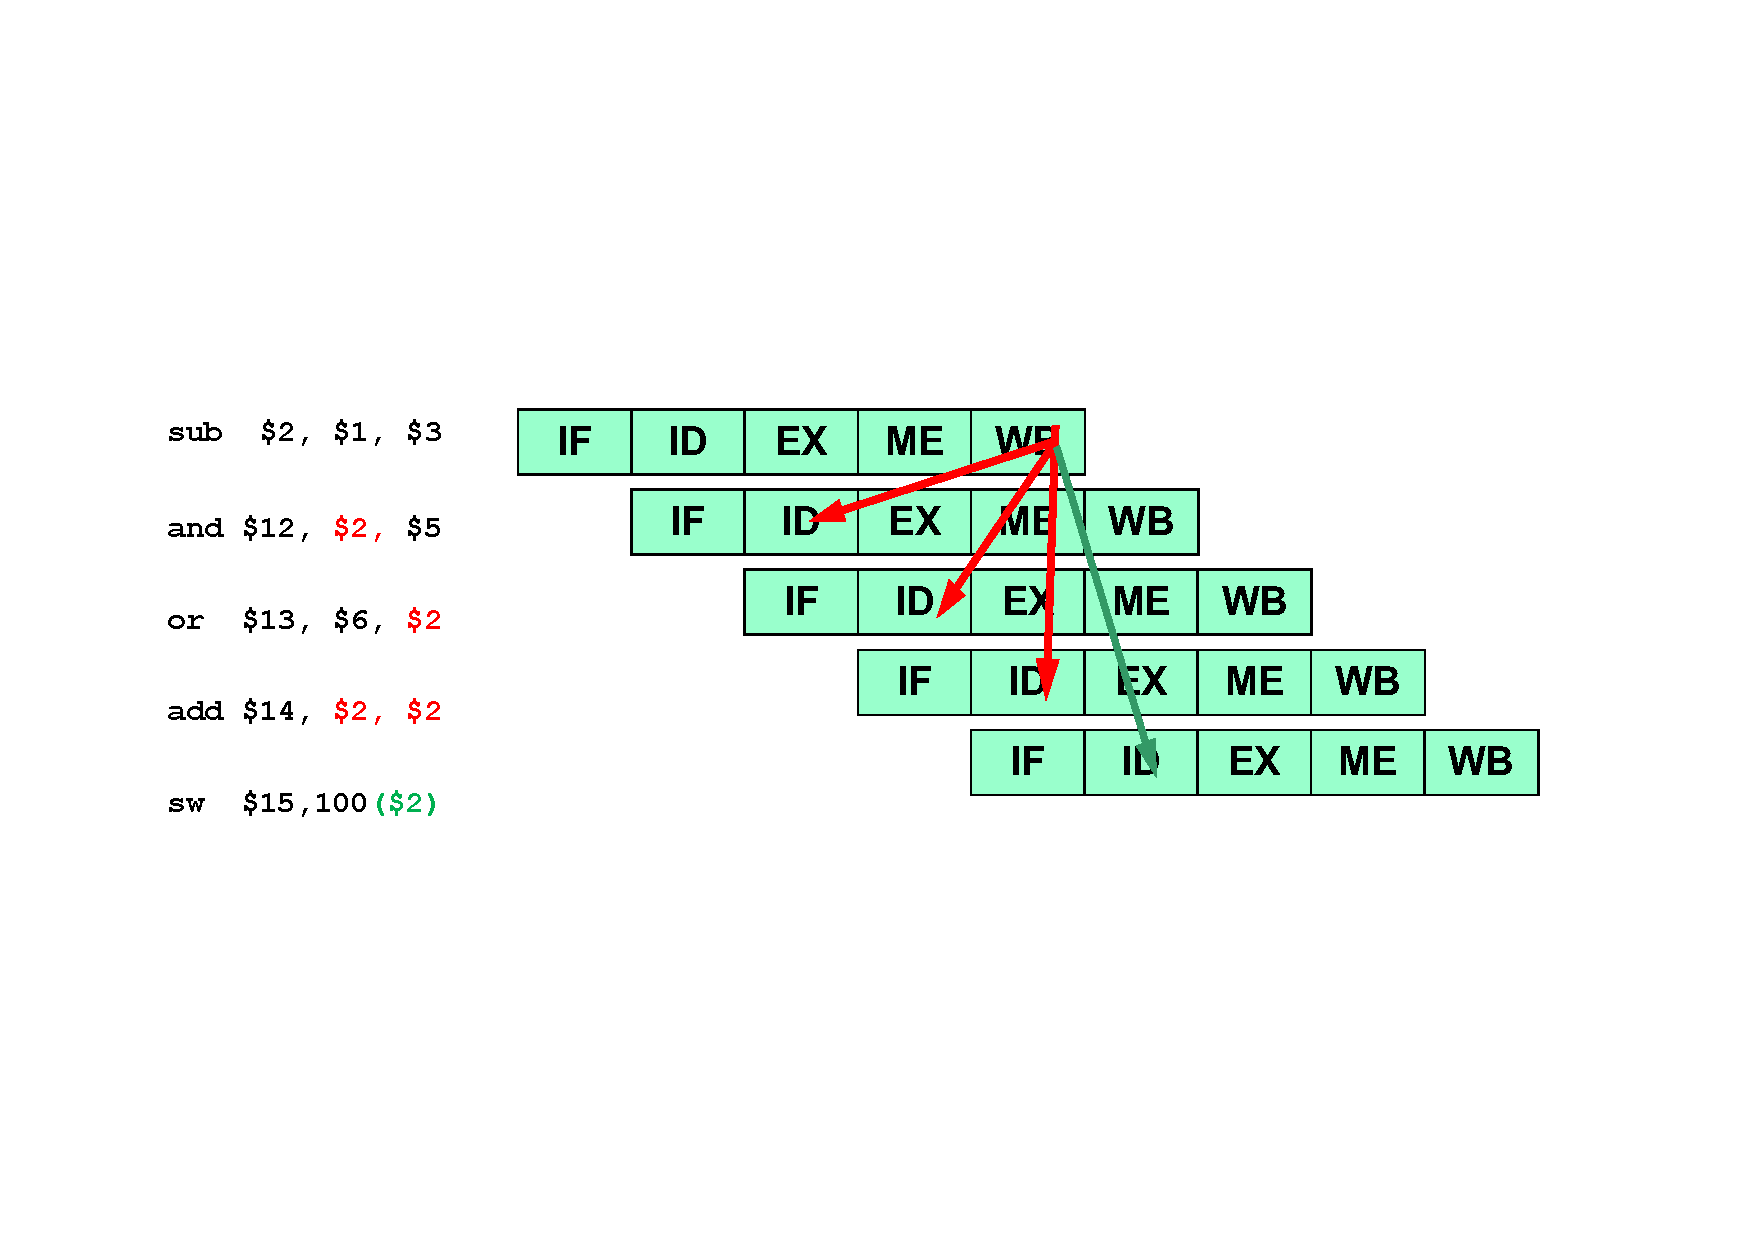
\includegraphics[width=\textwidth]{img/RAW-hazards-1.pdf}
    \caption{Why MIPS Optimized Pipeline was born.\cite{pipelining-slides}}
\end{figure}

\noindent
The Register File is used in 2 stages: read access during ID (\texttt{and} operation) and write access during Write Back (WB) (\texttt{sub} operation). \emph{What happens if read and write refer to the same register in the same clock cycle?} Or we insert a stall, or we use an \textbf{optimized pipeline} (smart choice).

\begin{definitionbox}[: Optimized Pipeline]
    By selecting \definition{Optimized Pipeline}, we assume the Register File (RF) read occurs in the second half of clock cycle and the Register File write in the first half of clock cycle.
\end{definitionbox}

\noindent
This way \textbf{we don't need the stall}. The following Figure~\ref{fig: Optimized Pipeline} shows an optimized pipeline.

\newpage

\begin{figure}[!htp]
    \centering
    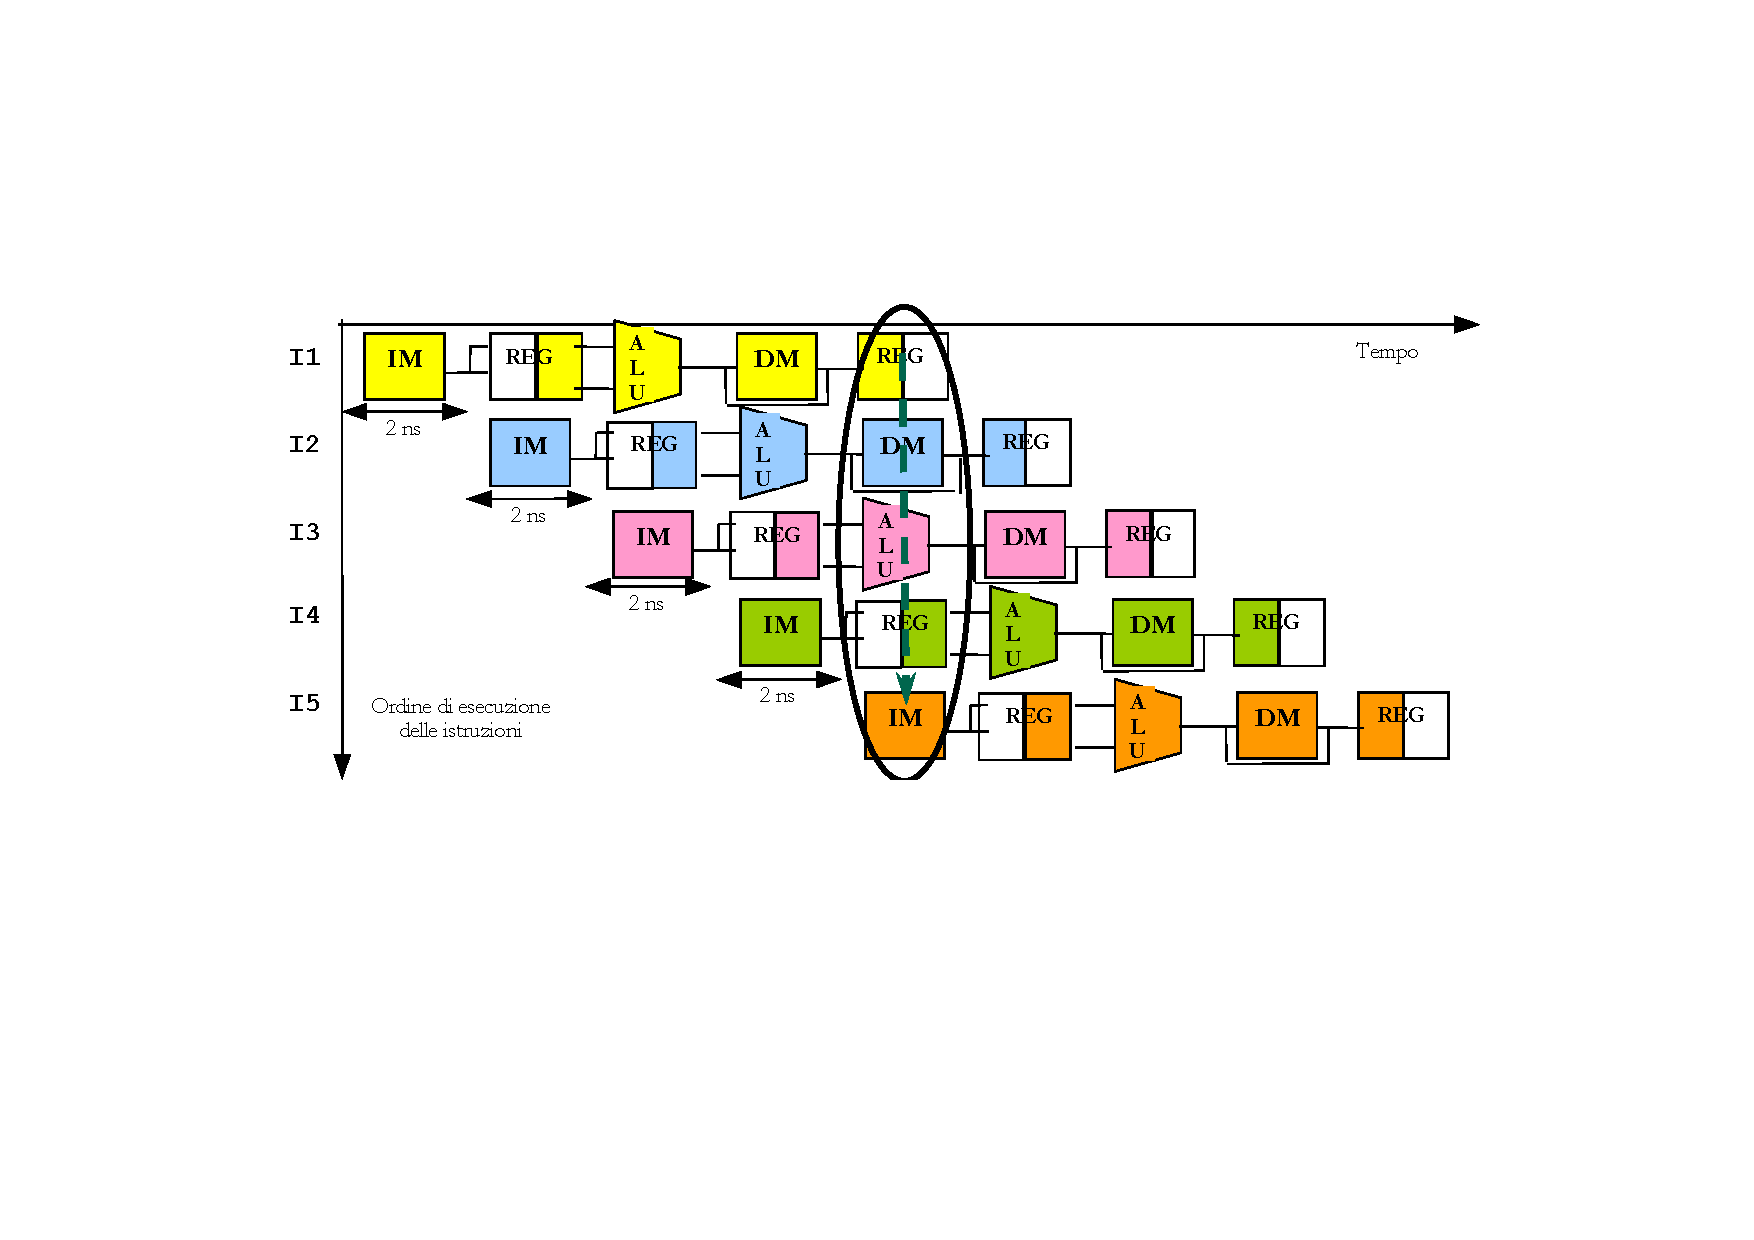
\includegraphics[width=\textwidth]{img/optimized-pipeline-1.pdf}
    \caption{Optimized Pipeline (IM is Instruction Memory, REG is Register File, and DM is Data Memory).\cite{pipelining-slides}}
    \label{fig: Optimized Pipeline}
\end{figure}

\noindent
And the problem mentioned at the beginning of this paragraph is partially solved, as we can see in the following figure.
\begin{figure}[!htp]
    \centering
    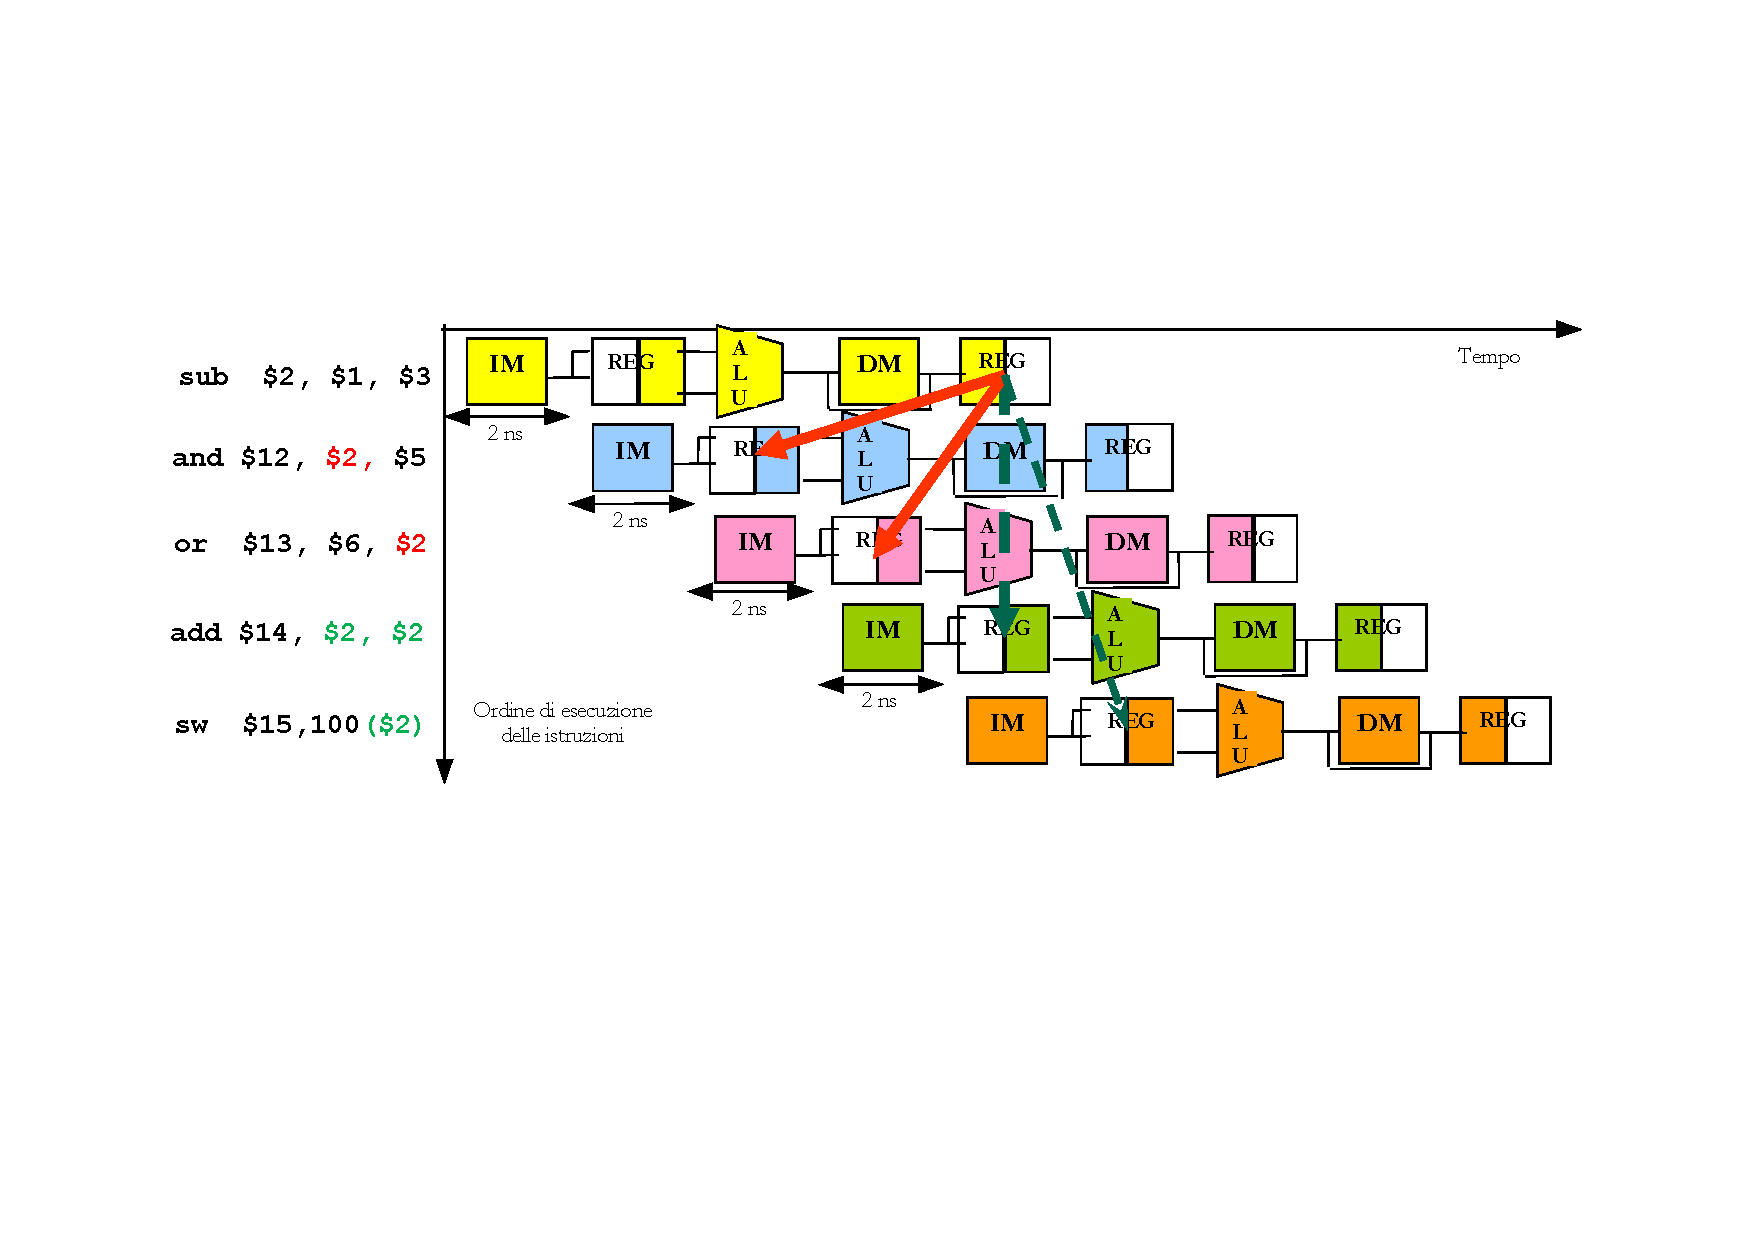
\includegraphics[width=\textwidth]{img/optimized-pipeline-2.pdf}
    \caption{Optimized Pipeline to solve the example stall.\cite{pipelining-slides}}
\end{figure}
    \subsubsection{The solution of Data Hazards}

The following techniques don't solve the problem completely, but they do solve it partially. So they find a perfect balance between the ideal speedup and a situation where the hazard is total.

\highspace
The solution can be applied on runtime (hardware techniques) or on compilation (static-time techniques):
\begin{itemize}
    \item \textbf{Compilation Techniques} (static-time techniques):
    \begin{itemize}
        \item The \definition{insertion of \texttt{nop}} is a simple (logical) solution where we \textbf{insert a \texttt{nop} operator between dependent statements} to ensure correct operation.

        See the \example{example} on page \pageref{example: insertion of nop}.


        \item The \definition{instructions scheduling} is a technique used by the compiler to prevent correlating instructions from being too close together. It tries to \textbf{reorder instructions} by inserting independent instructions between correlating instructions. \textbf{If the compiler can't do this, it inserts \texttt{nop} operations}.

        See the \example{example} on page \pageref{example: instructions scheduling}.
    \end{itemize}

    \item \textbf{Hardware Techniques} (runtime techniques):
    \begin{itemize}
        \item The \definition{insertion of stalls} (called also \emph{bubbling the pipeline}, \emph{pipeline break}, or \emph{pipeline stall}) is a sort of a delay before the processor can resume execution of the instruction. As we can see in the \example{example} on page \pageref{example: insertion of stalls}, the stalls delay the stages of the correlating instructions.

        \item The \definition{data forwarding} \textbf{uses temporary results stored in the pipeline registers} instead of waiting for the results to be written back to the Register File (RF). To do this, it's \textbf{necessary to add new paths and multiplexers at the inputs of the ALU} to fetch inputs from the pipeline to avoid inserting stalls in the pipeline.

        See the \example{example} on page \pageref{example: data forwarding}.
    \end{itemize}
\end{itemize}
We have the mandatory to give more words to the data forwarding technique. First of all, its implementation needs new paths and new multiplexers. So, to adapt the MIPS architecture, the new implementation will be show in the figure \ref{fig: implementation of MIPS with Forwarding Unit} on page \pageref{fig: implementation of MIPS with Forwarding Unit}.

\newpage

\begin{figure}[!htp]
    \centering
    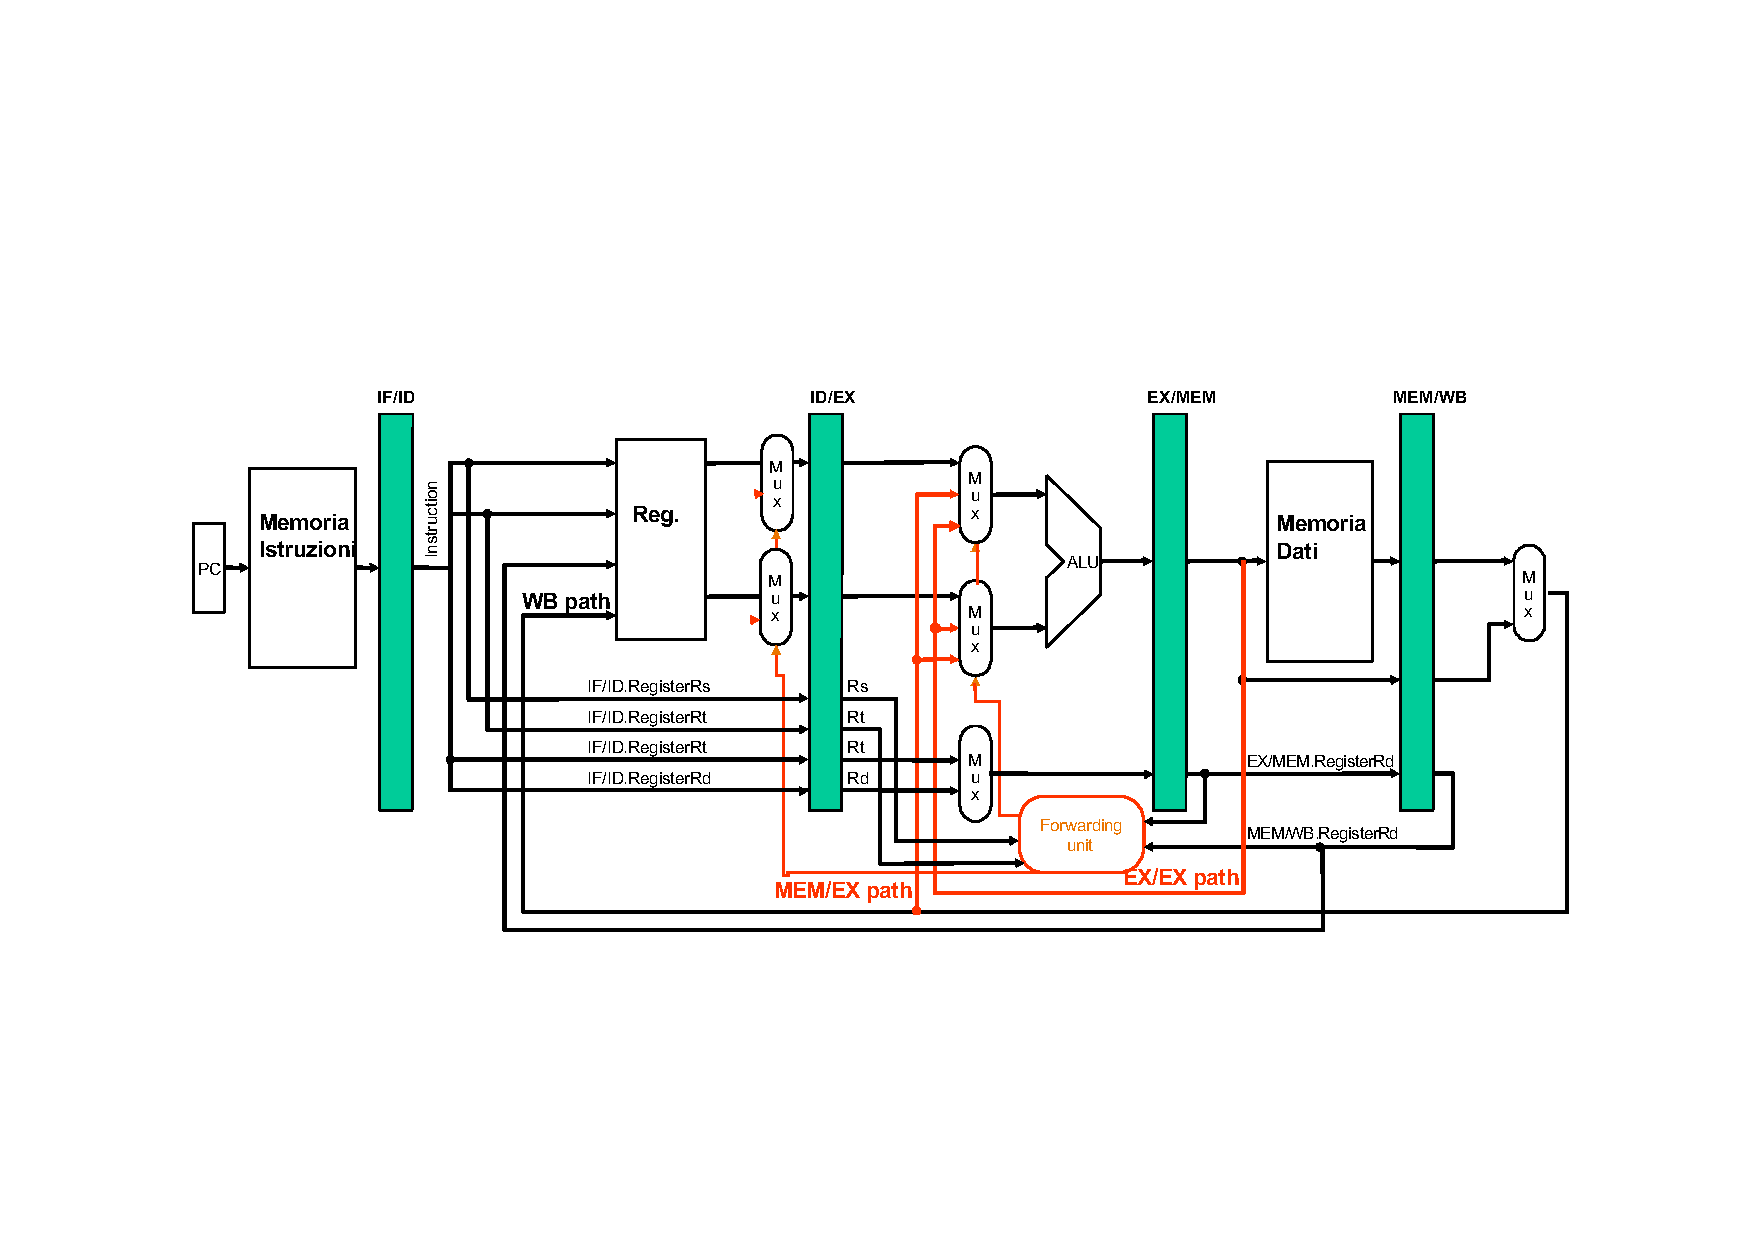
\includegraphics[width=\textwidth]{img/implementation-mips-forwarding-unit-1.pdf}
    \caption{Implementation of MIPS with \definition{Forwarding Unit}.\cite{pipelining-slides}}
    \label{fig: implementation of MIPS with Forwarding Unit}
\end{figure}

\noindent
Scan (or click) the QR code below to view the figure~\ref{fig: implementation of MIPS with Forwarding Unit} in high quality:
\begin{center}
    \qrcode{https://github.com/PoliMI-HPC-E-notes-projects-AndreVale69/HPC-E-PoliMI-university-notes/tree/main/advanced-computer-architectures/notes/img/implementation-mips-forwarding-unit-1.pdf}
\end{center}

\noindent
The forwarding paths created inside the MIPS architecture are three: \textbf{\texttt{EX} to \texttt{EX}} path, \textbf{\texttt{MEM} to \texttt{EX}} path, and \textbf{\texttt{MEM} to \texttt{MEM}} path.
\begin{figure}[!htp]
    \centering
    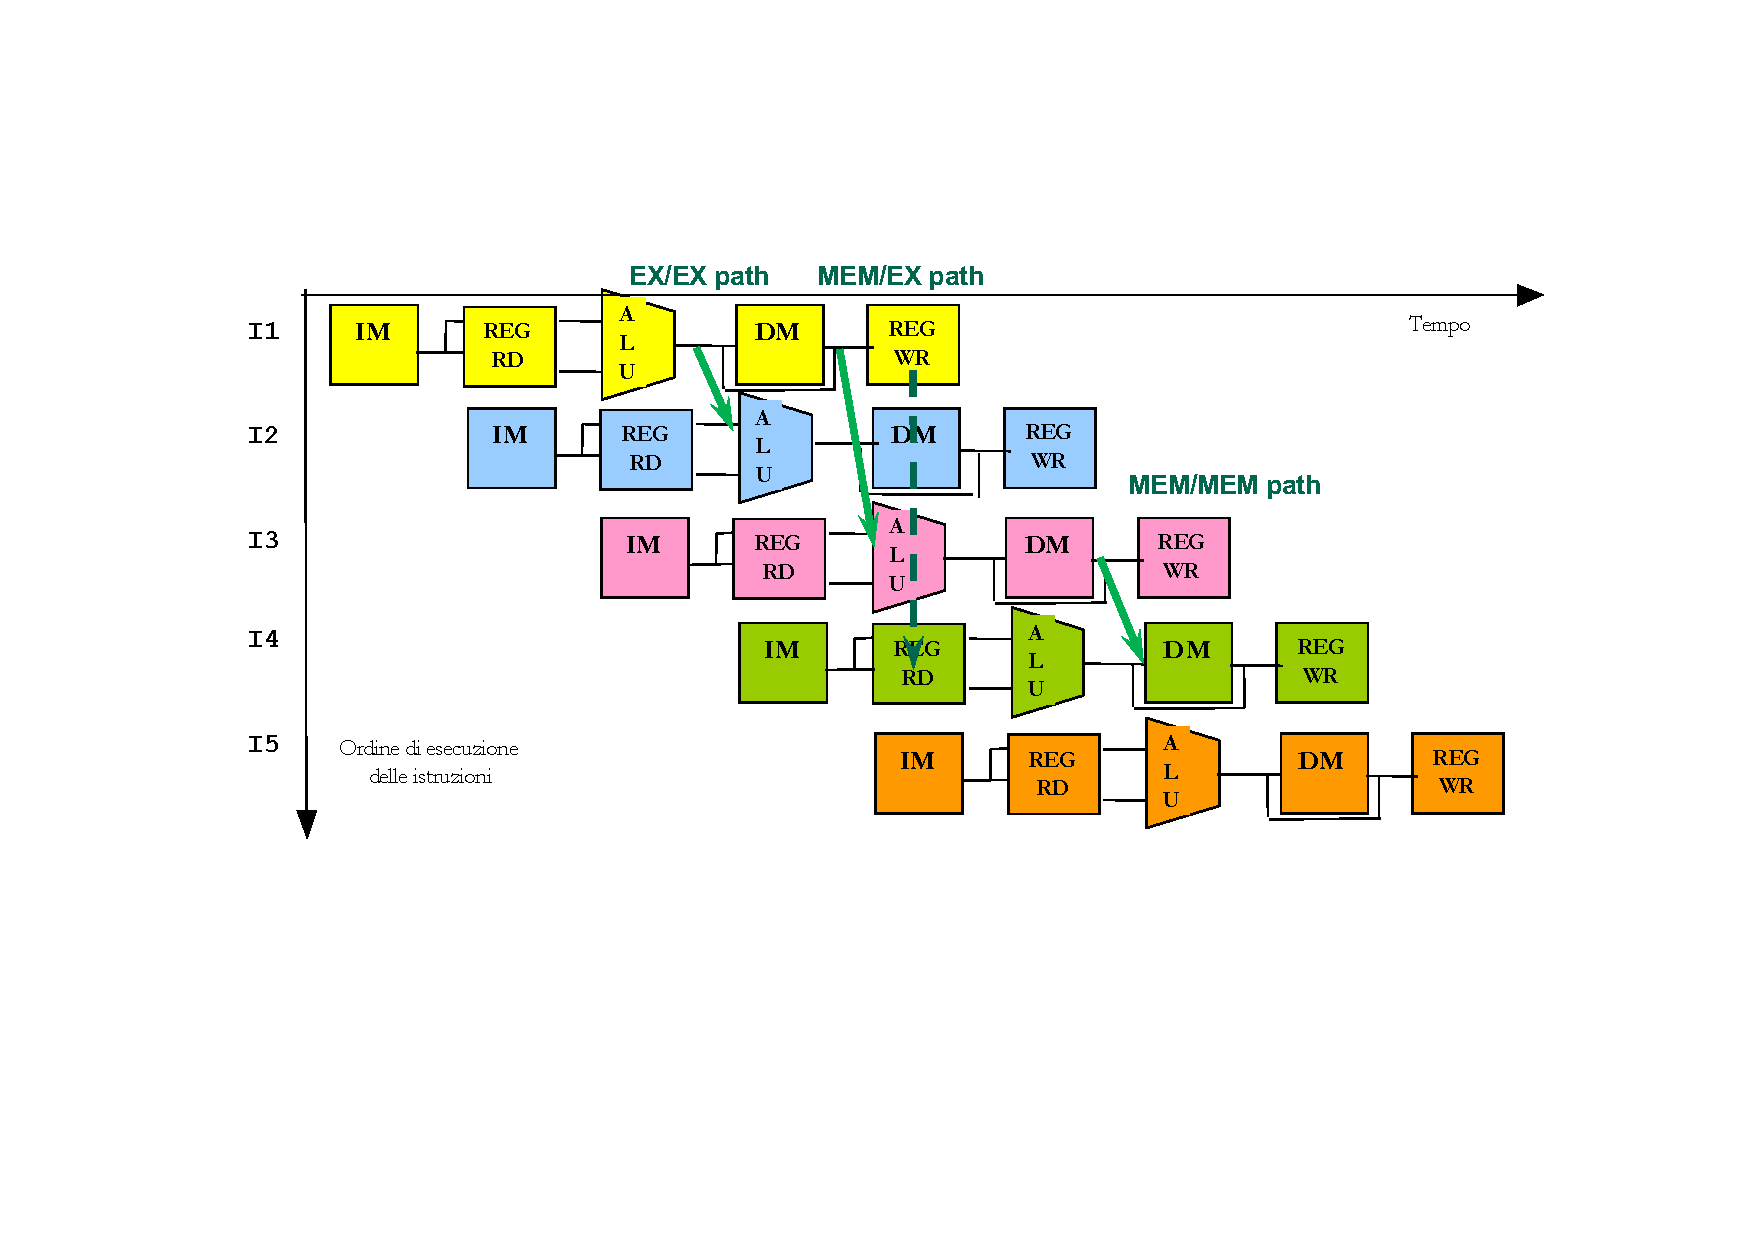
\includegraphics[width=\textwidth]{img/forwarding-paths-1.pdf}
    \caption{Forwarding paths on MIPS architecture.\cite{pipelining-slides}}
\end{figure}

\noindent
Furthermore, the \textbf{forwarding technique can solve} the \textbf{Load-Use} and \textbf{Load-Store} Data Hazard. It's a very interesting feature because the \texttt{MEM} to \texttt{EX} and \texttt{MEM} to \texttt{MEM} paths can solve two different situations:
\begin{itemize}
    \item \textbf{Load-Use} Hazard. It's \textbf{solved by MEM to EX path} because the value loaded in the MEM stage, is forwarded directly to the EX stage of the next conflict instruction (but unfortunately we need one stall to delay the run).

    \begin{examplebox}
        Given the following code:
        \lstinputlisting[language=misc]{code/solution-of-data-hazards/load-use-hazard-1.s}
        The \texttt{s0} operand depends on the load (\texttt{lw}) operator. Here, the problem of \textbf{\emph{load-use hazard}} occurs.
        \begin{center}
            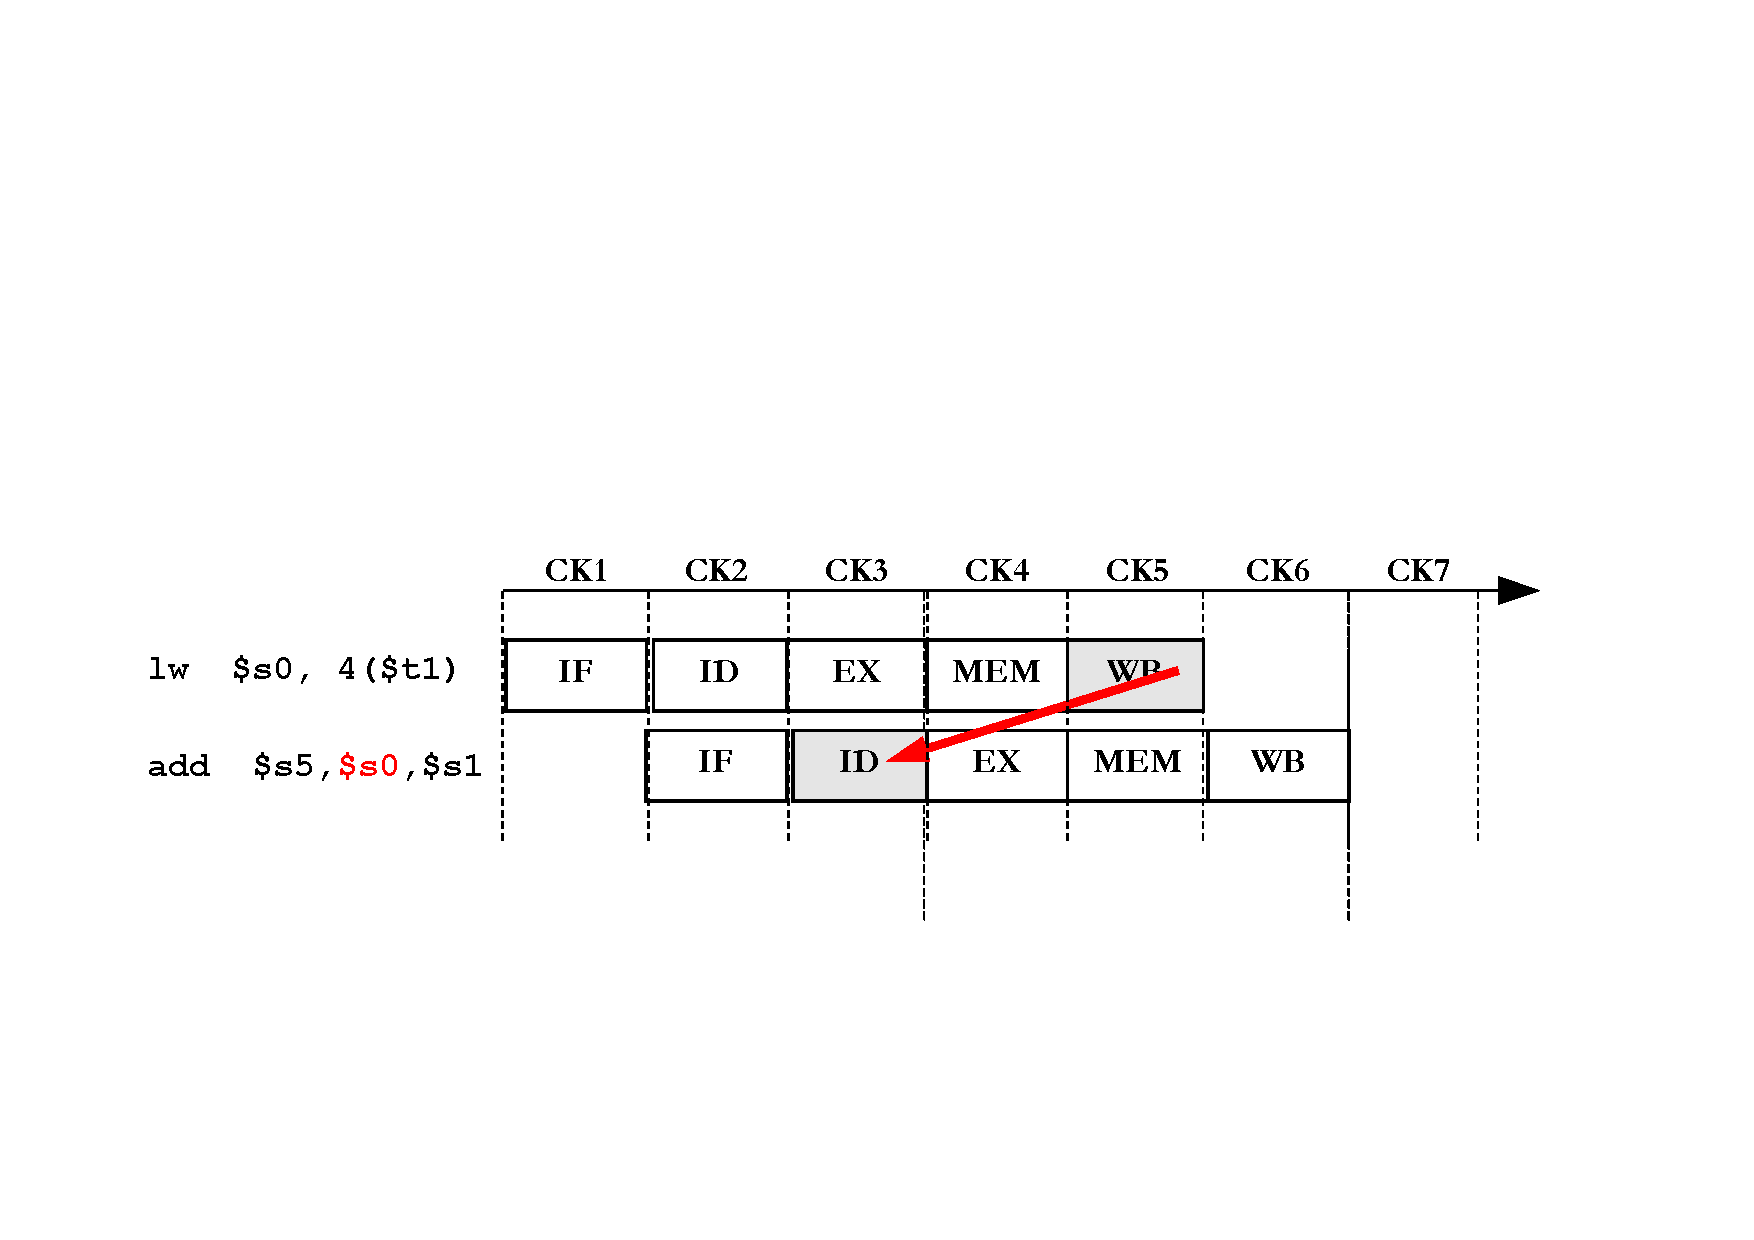
\includegraphics[width=\textwidth]{img/load-use-hazard-problem-1.pdf}
            \captionof*{figure}{The load-use hazard problem.\cite{pipelining-slides}}
        \end{center}
        In the figure, we can see the existing dependence. An ideal solution to the load-use hazard should be taking the value after the Memory Access operation (because the load instruction reads the effective address on the memory) and using it in the sum (operation).

        The \textbf{forwarding technique solves it using the MEM-EX path but using \underline{one stall}}.
        \begin{center}
            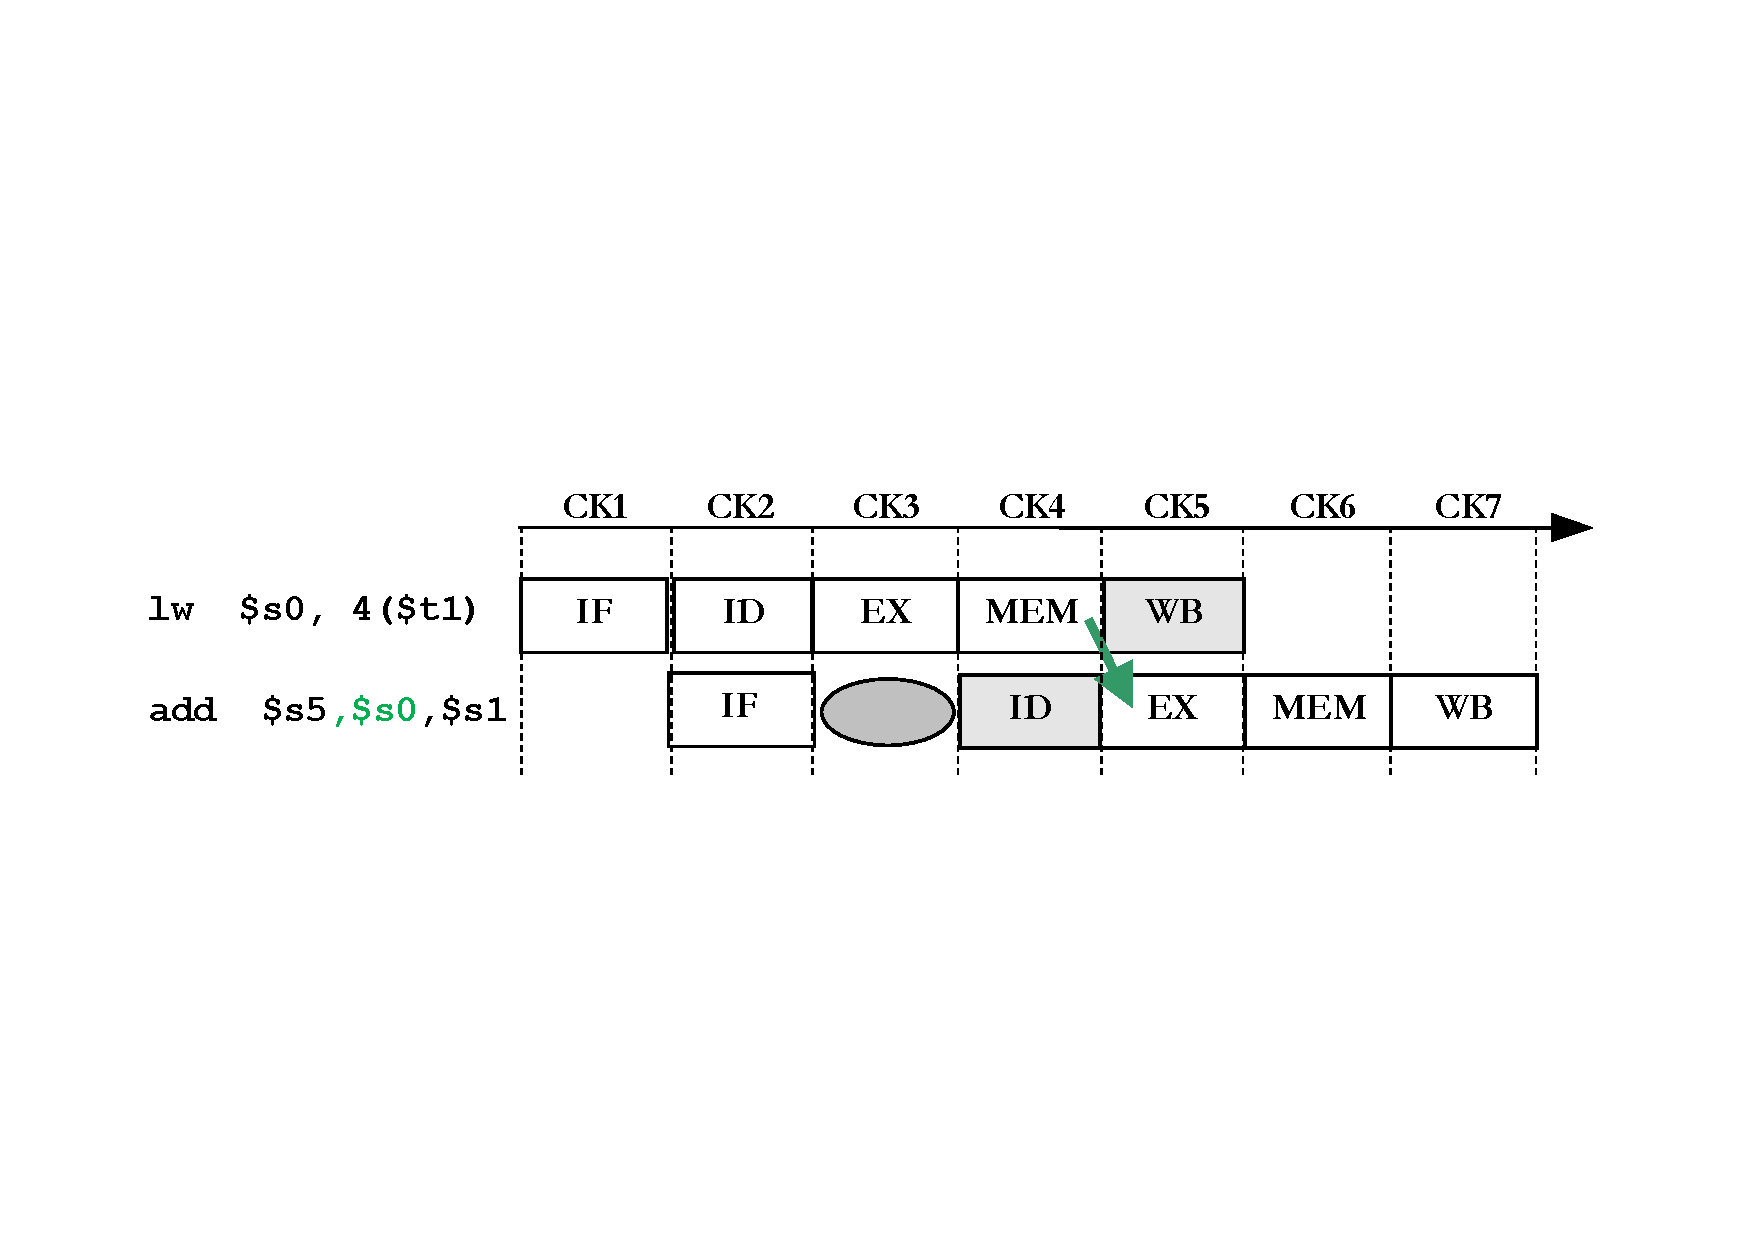
\includegraphics[width=\textwidth]{img/load-use-hazard-problem-2.pdf}
            \captionof*{figure}{Forwarding technique with MEM-EX path.\cite{pipelining-slides}}
        \end{center}
    \end{examplebox}
    % TODO: add example

    \item \textbf{Load-Store} Hazard. It's \textbf{solved by MEM to MEM path} because the value loaded in the MEM stage, is forwarded directly to the MEM stage of the next conflict instruction.
    \begin{examplebox}
        Given the following code:
        \lstinputlisting[language=misc]{code/solution-of-data-hazards/load-store-hazard-1.s}
        The \texttt{s0} operand depends on the load (\texttt{lw}) operator. Here, the problem of \textbf{\emph{load-store hazard}} occurs.
        \begin{center}
            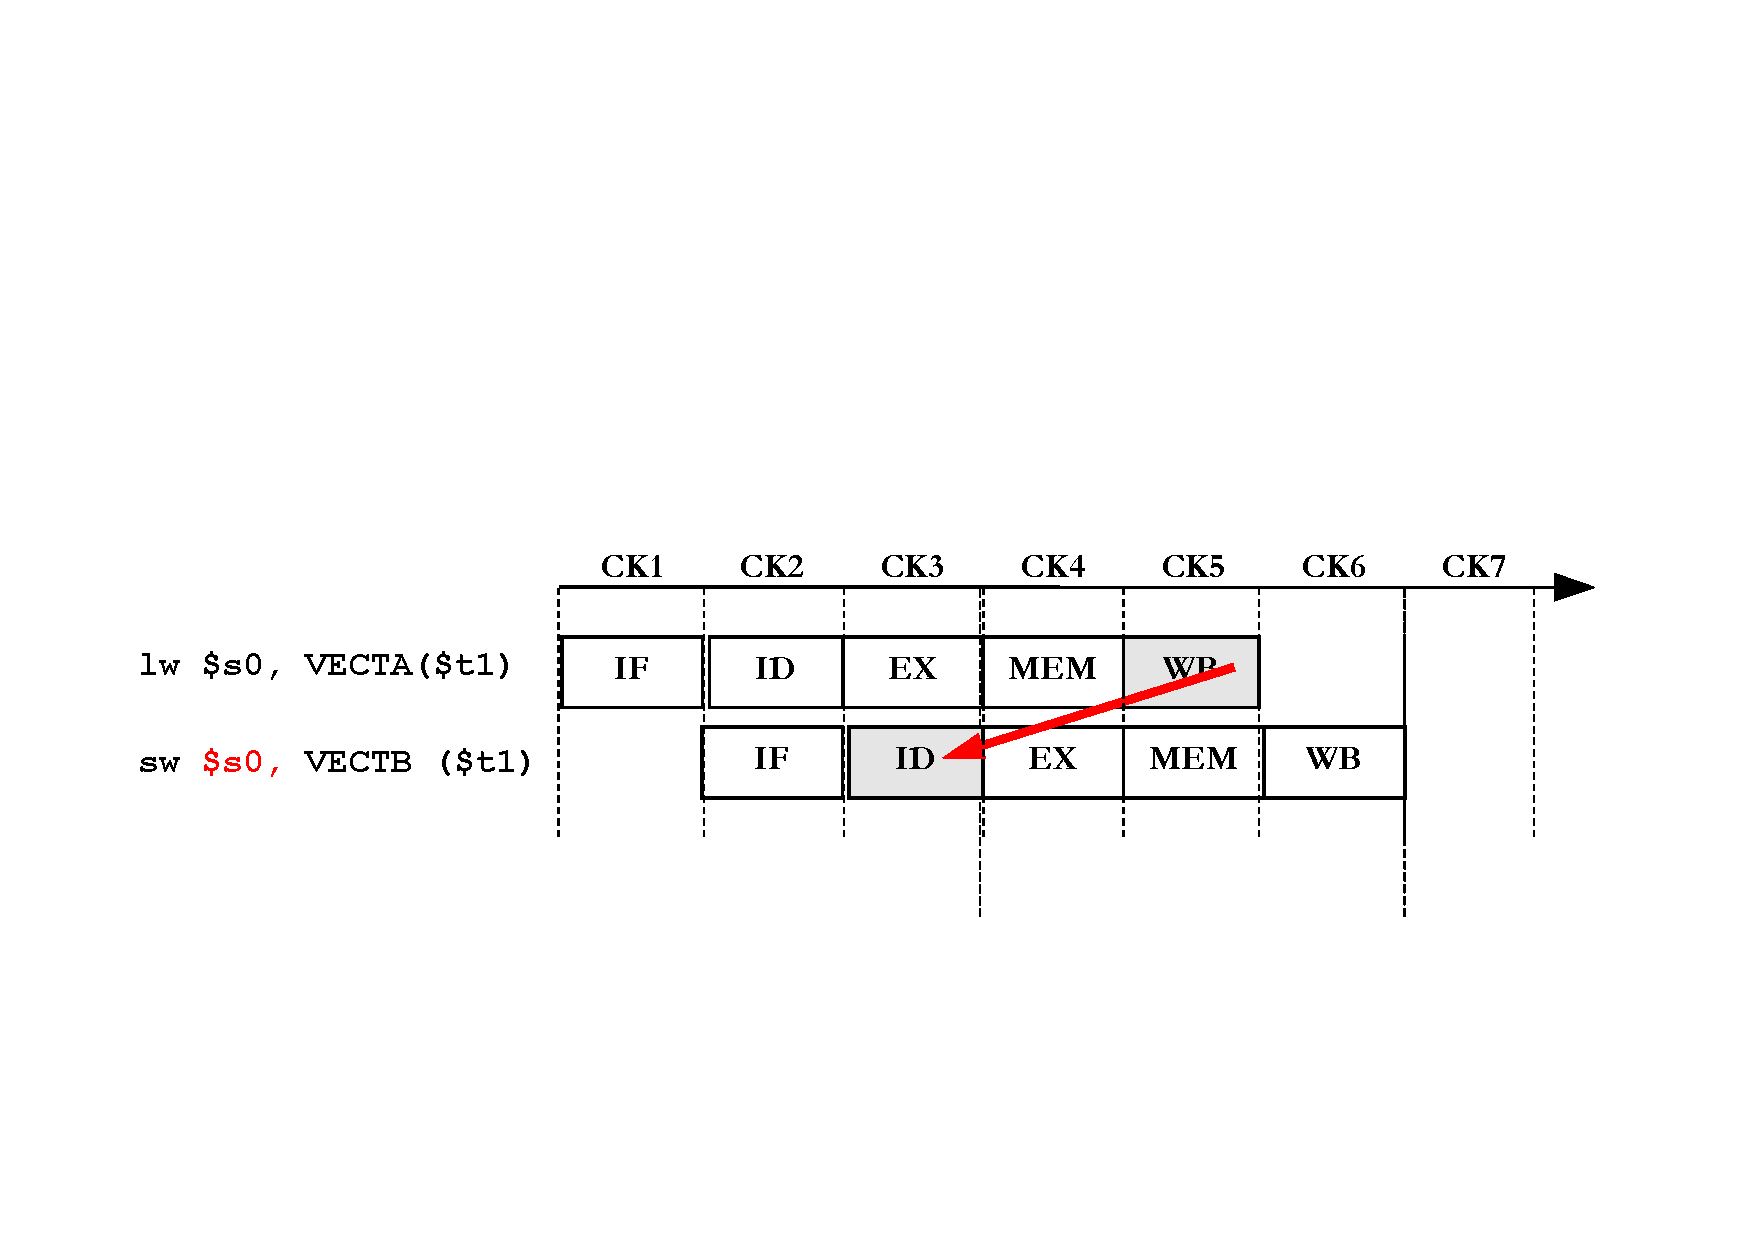
\includegraphics[width=\textwidth]{img/load-store-hazard-problem-1.pdf}
            \captionof*{figure}{The load-store hazard problem.\cite{pipelining-slides}}
        \end{center}
        In the figure, we can see the existing dependence. An ideal solution to the load-store hazard should be taking the value after the Write Back operation (because the load instruction writes the data read from memory in the destination register of the Register File) and using it in the Instruction Decode (because the ID includes also Register Read, then it reads from the Register File (RF)).

        The \textbf{forwarding technique solves it using the MEM-MEM path \underline{without any stall}}.
        \begin{center}
            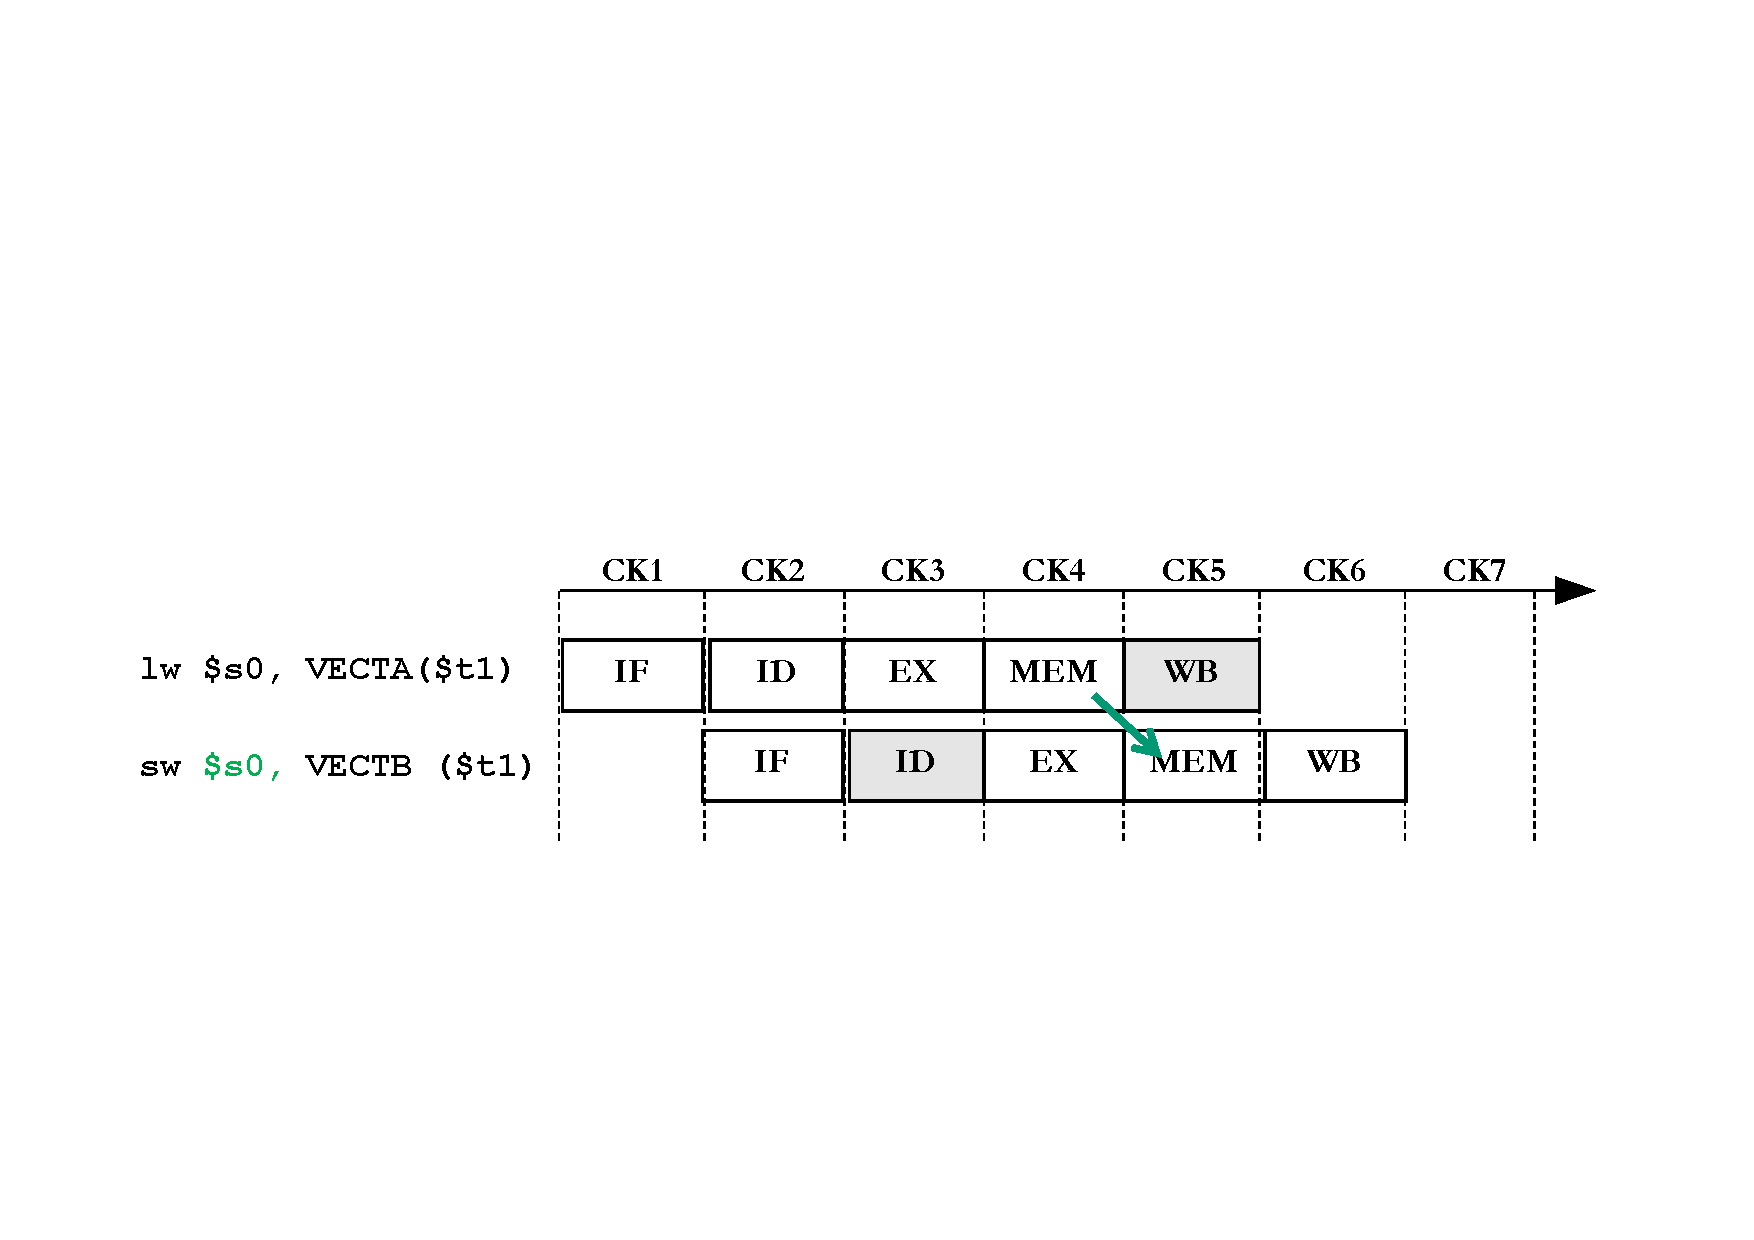
\includegraphics[width=\textwidth]{img/load-store-hazard-problem-2.pdf}
            \captionof*{figure}{Forwarding technique with MEM-MEM path.\cite{pipelining-slides}}
        \end{center}
    \end{examplebox}
\end{itemize}

\begin{examplebox}\label{example: insertion of nop}
    In the following figure, we can see how a \textbf{compilation technique}, the \textbf{insertion of \texttt{nop}}, can be solve the data hazard problem.
    \begin{center}
        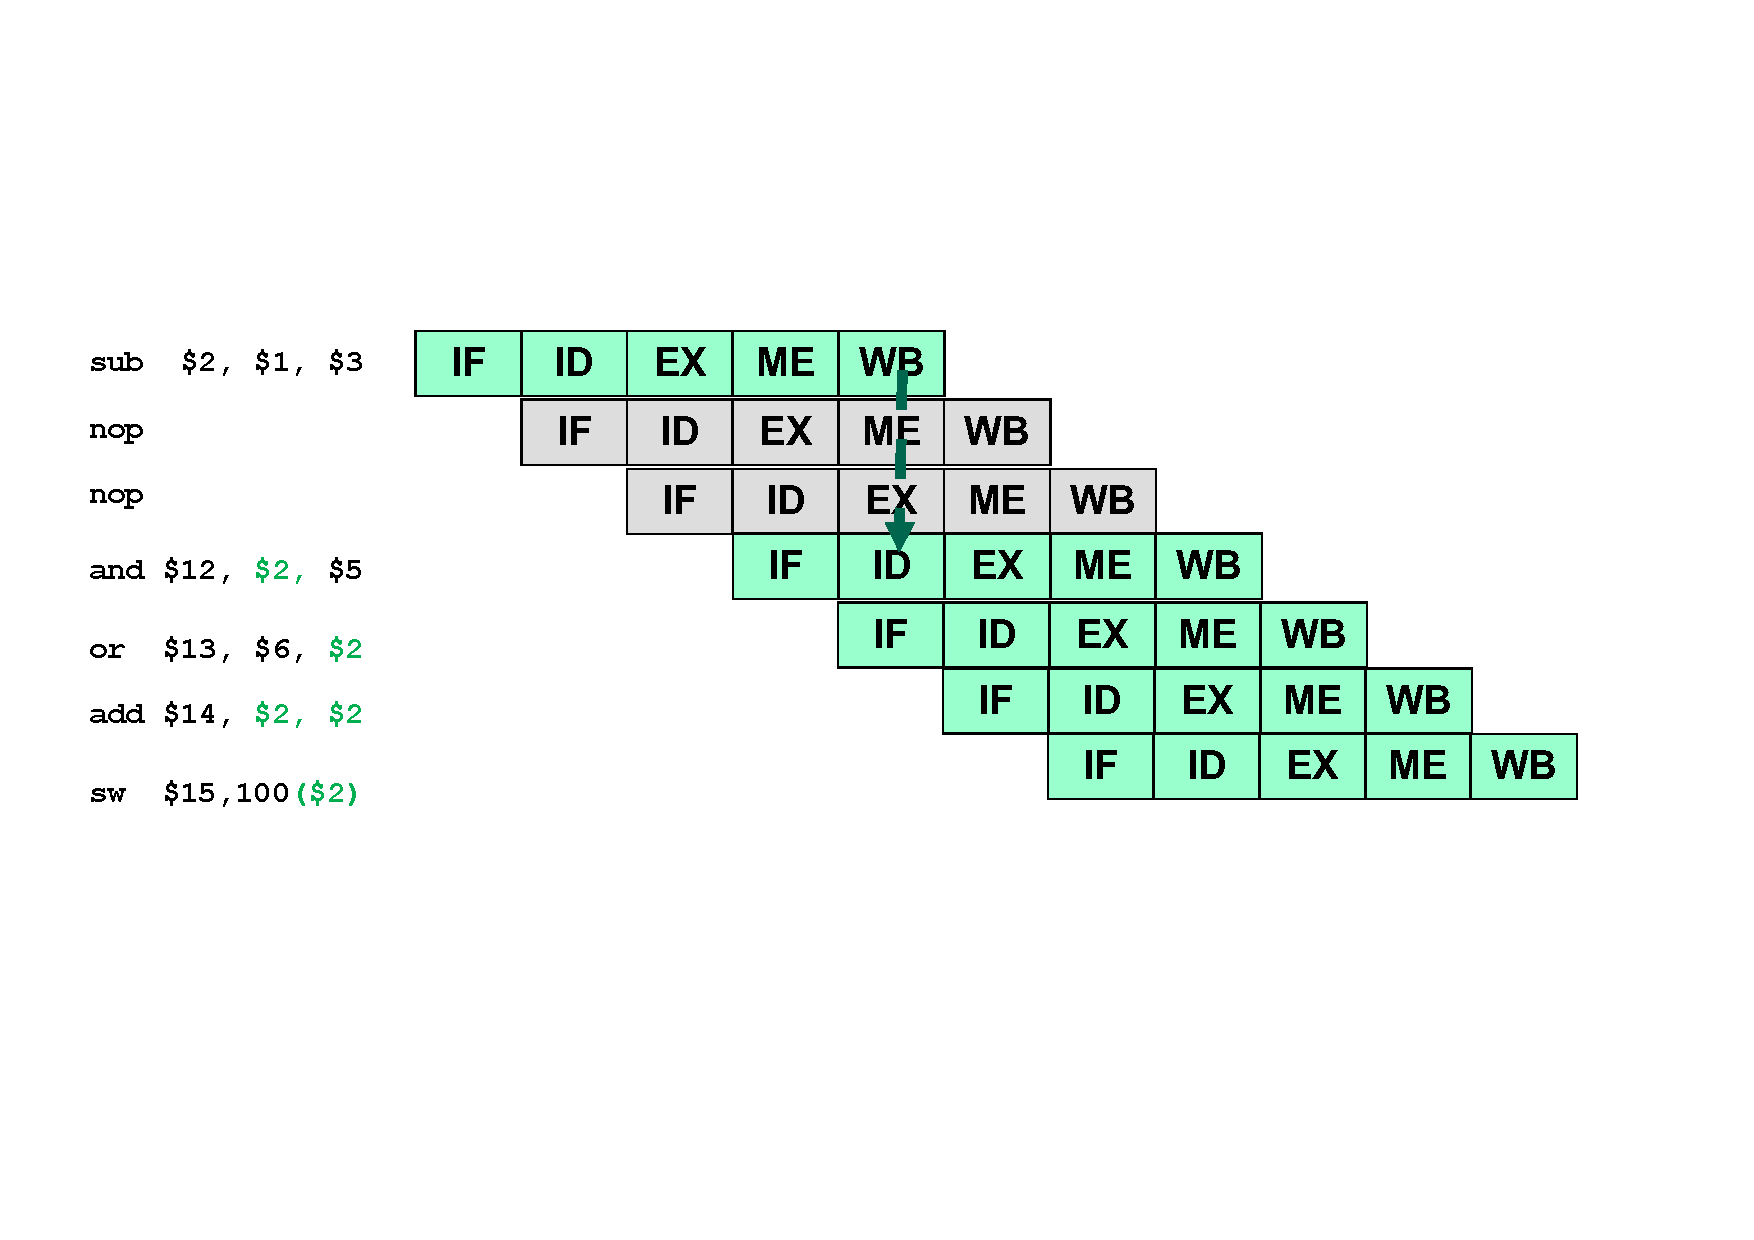
\includegraphics[width=\textwidth]{img/insertion-of-nop-1.pdf}
        \captionof*{figure}{Insertion of \texttt{nop}.\cite{pipelining-slides}}
    \end{center}
\end{examplebox}

\newpage

\begin{examplebox}\label{example: instructions scheduling}
    In the following figure, we can see how a \textbf{compilation technique}, the \textbf{instructions scheduling}, can be solve the data hazard problem.
    \begin{center}
        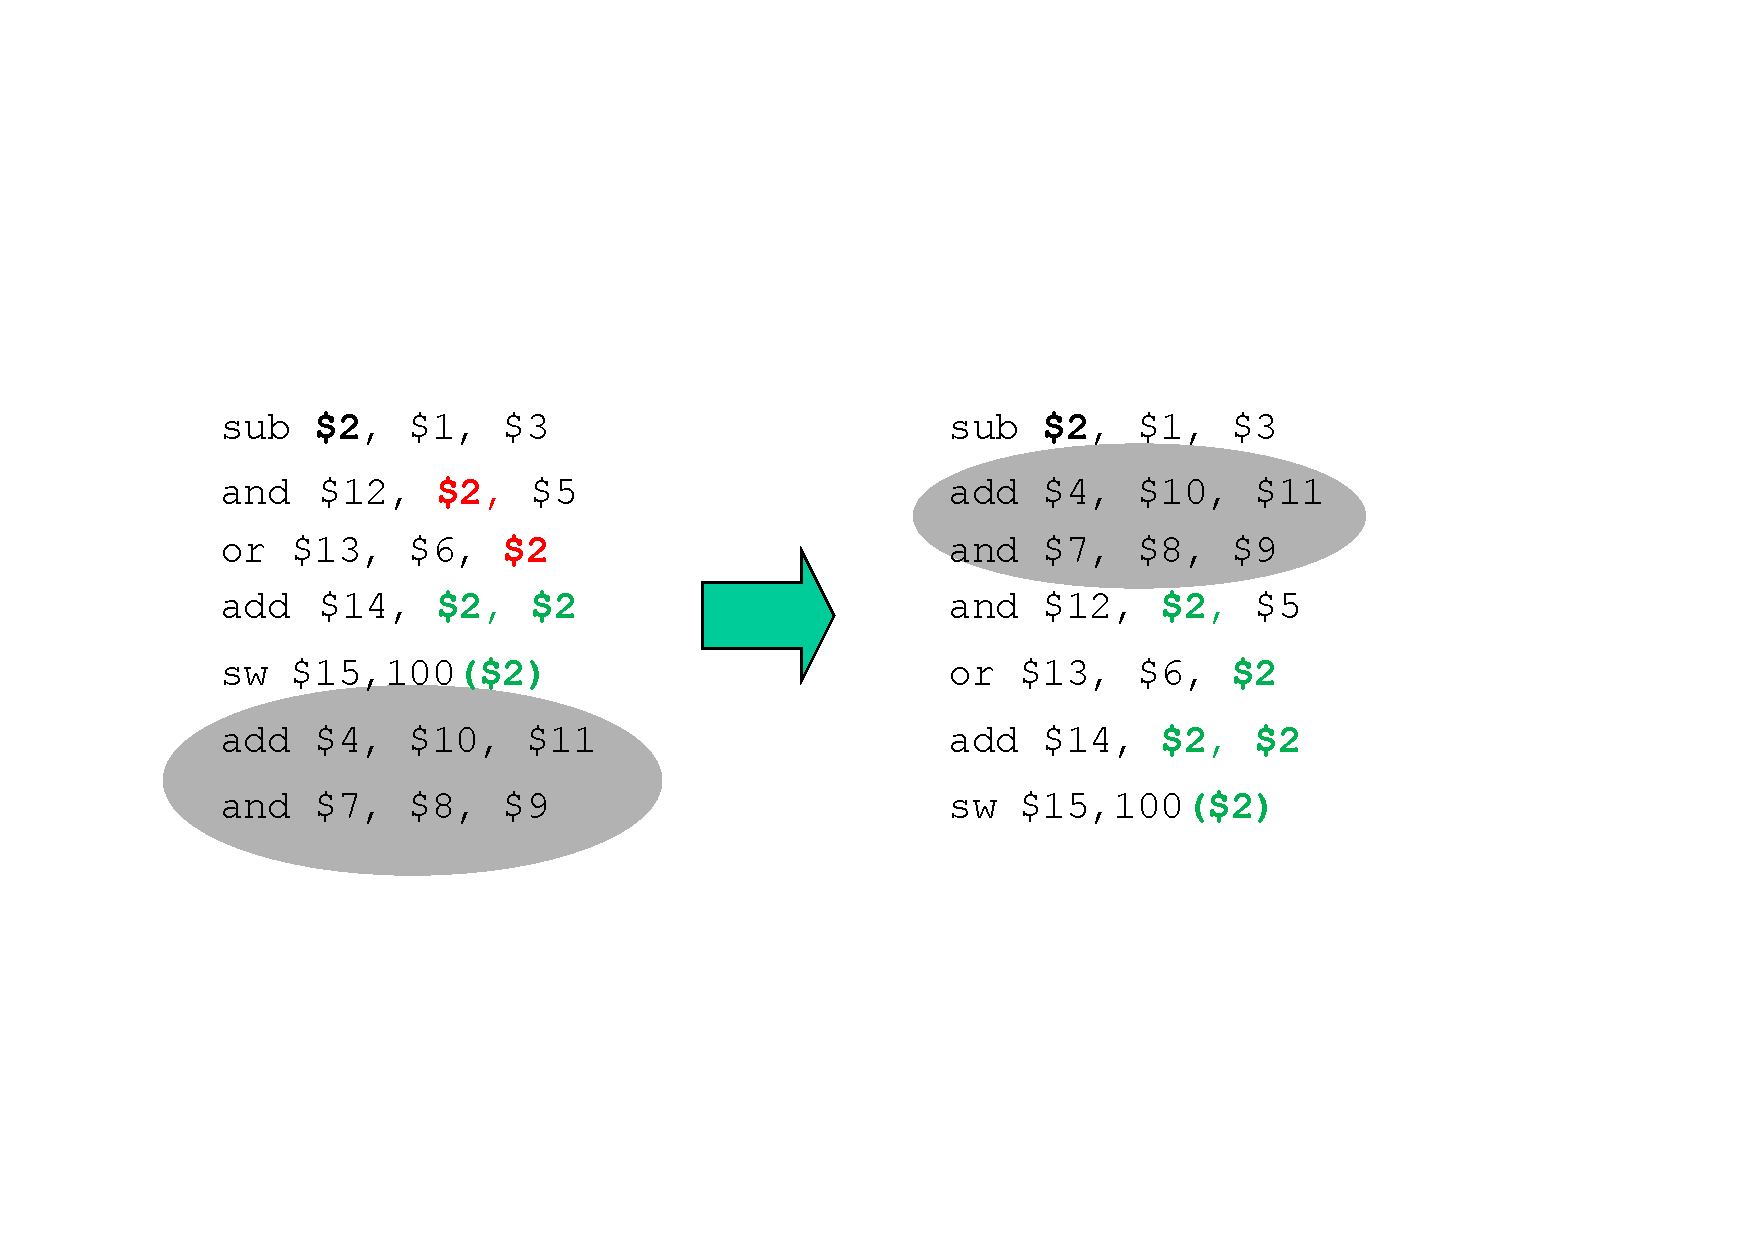
\includegraphics[width=\textwidth]{img/instructions-scheduling-1.pdf}
        \captionof*{figure}{Instructions scheduling.\cite{pipelining-slides}}
    \end{center}
\end{examplebox}

\begin{examplebox}\label{example: insertion of stalls}
    In the following figure, we can see how a \textbf{hardware technique}, the \textbf{insertion of stalls}, can be solve the data hazard problem.
    \begin{center}
        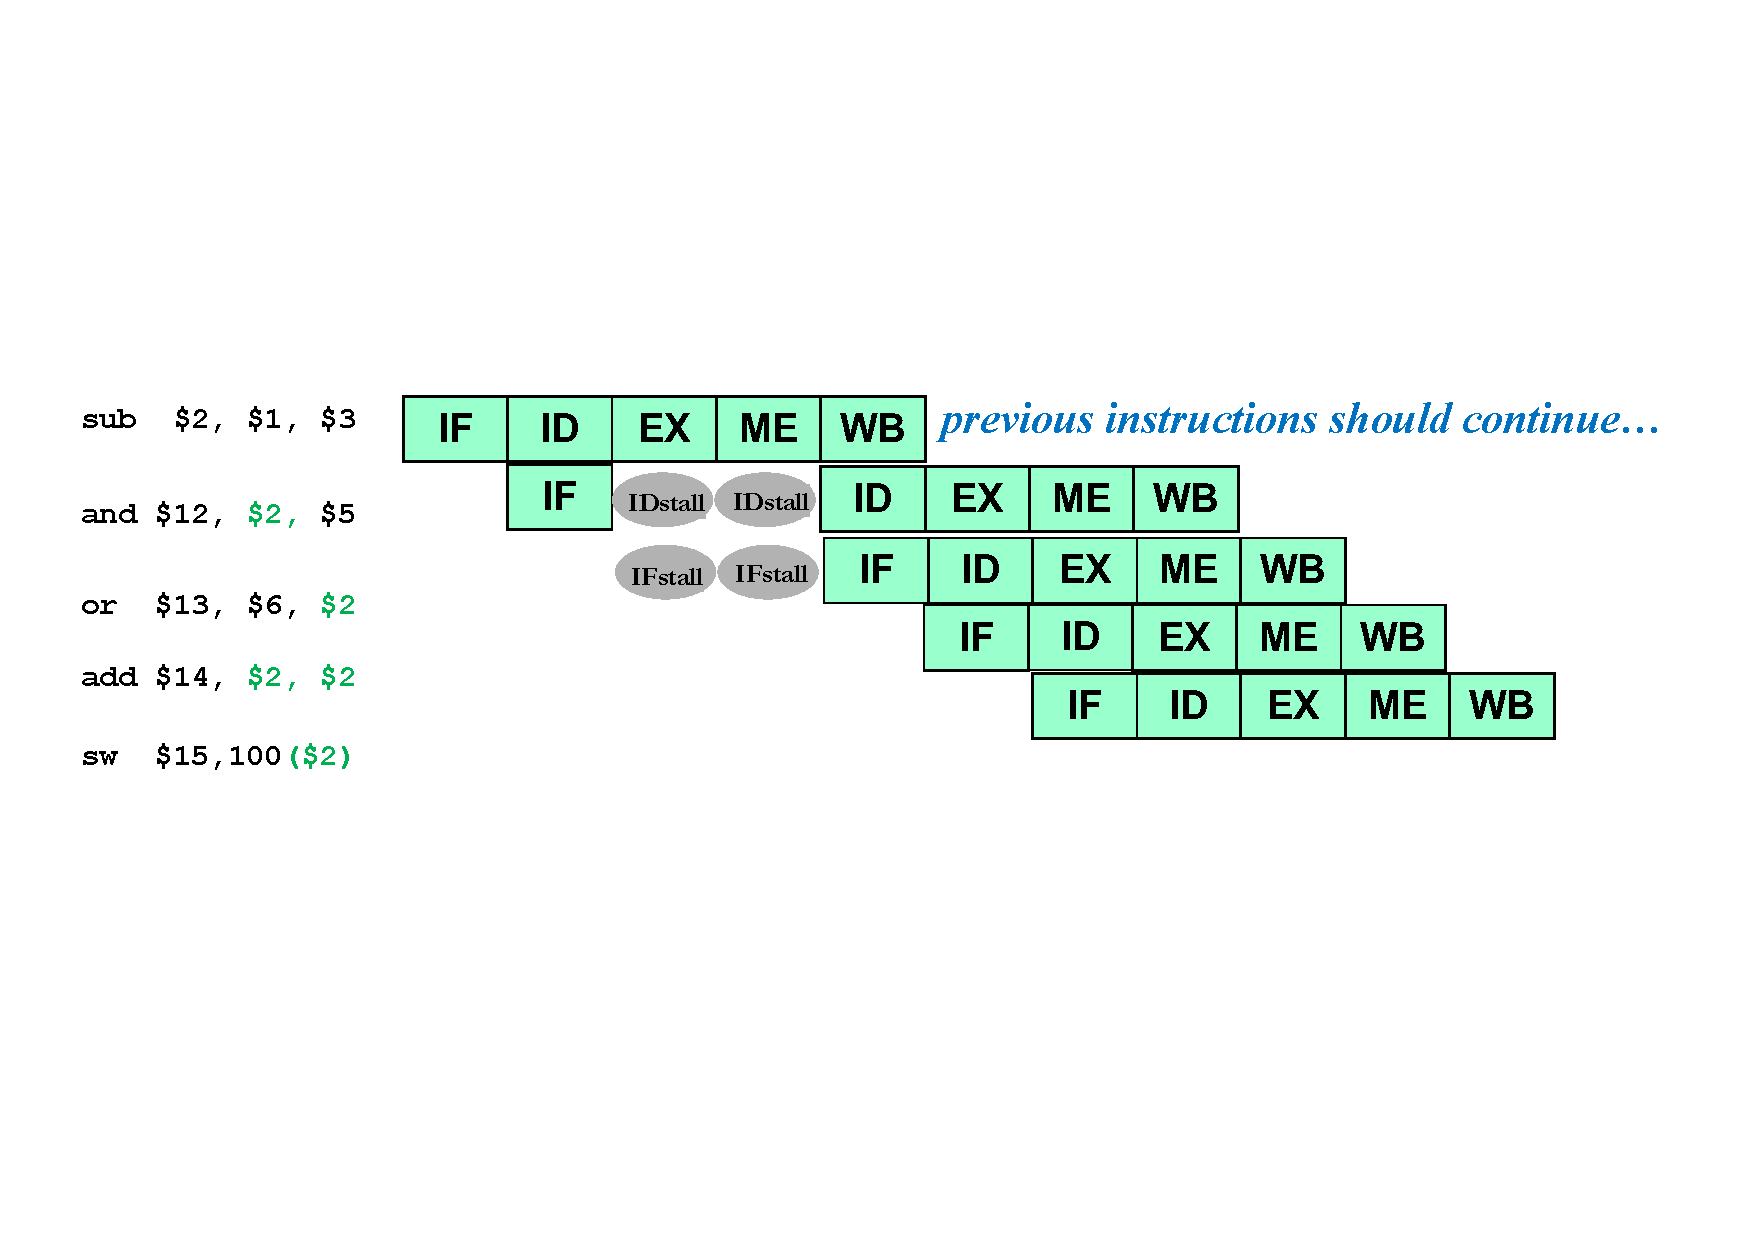
\includegraphics[width=\textwidth]{img/insertion-of-stalls-1.pdf}
        \captionof*{figure}{Insertion of stalls.\cite{pipelining-slides}}
    \end{center}
\end{examplebox}

\begin{examplebox}\label{example: data forwarding}
    In the following figure, we can see how a \textbf{hardware technique}, the \textbf{data forwarding}, can be solve the data hazard problem.
    \begin{center}
        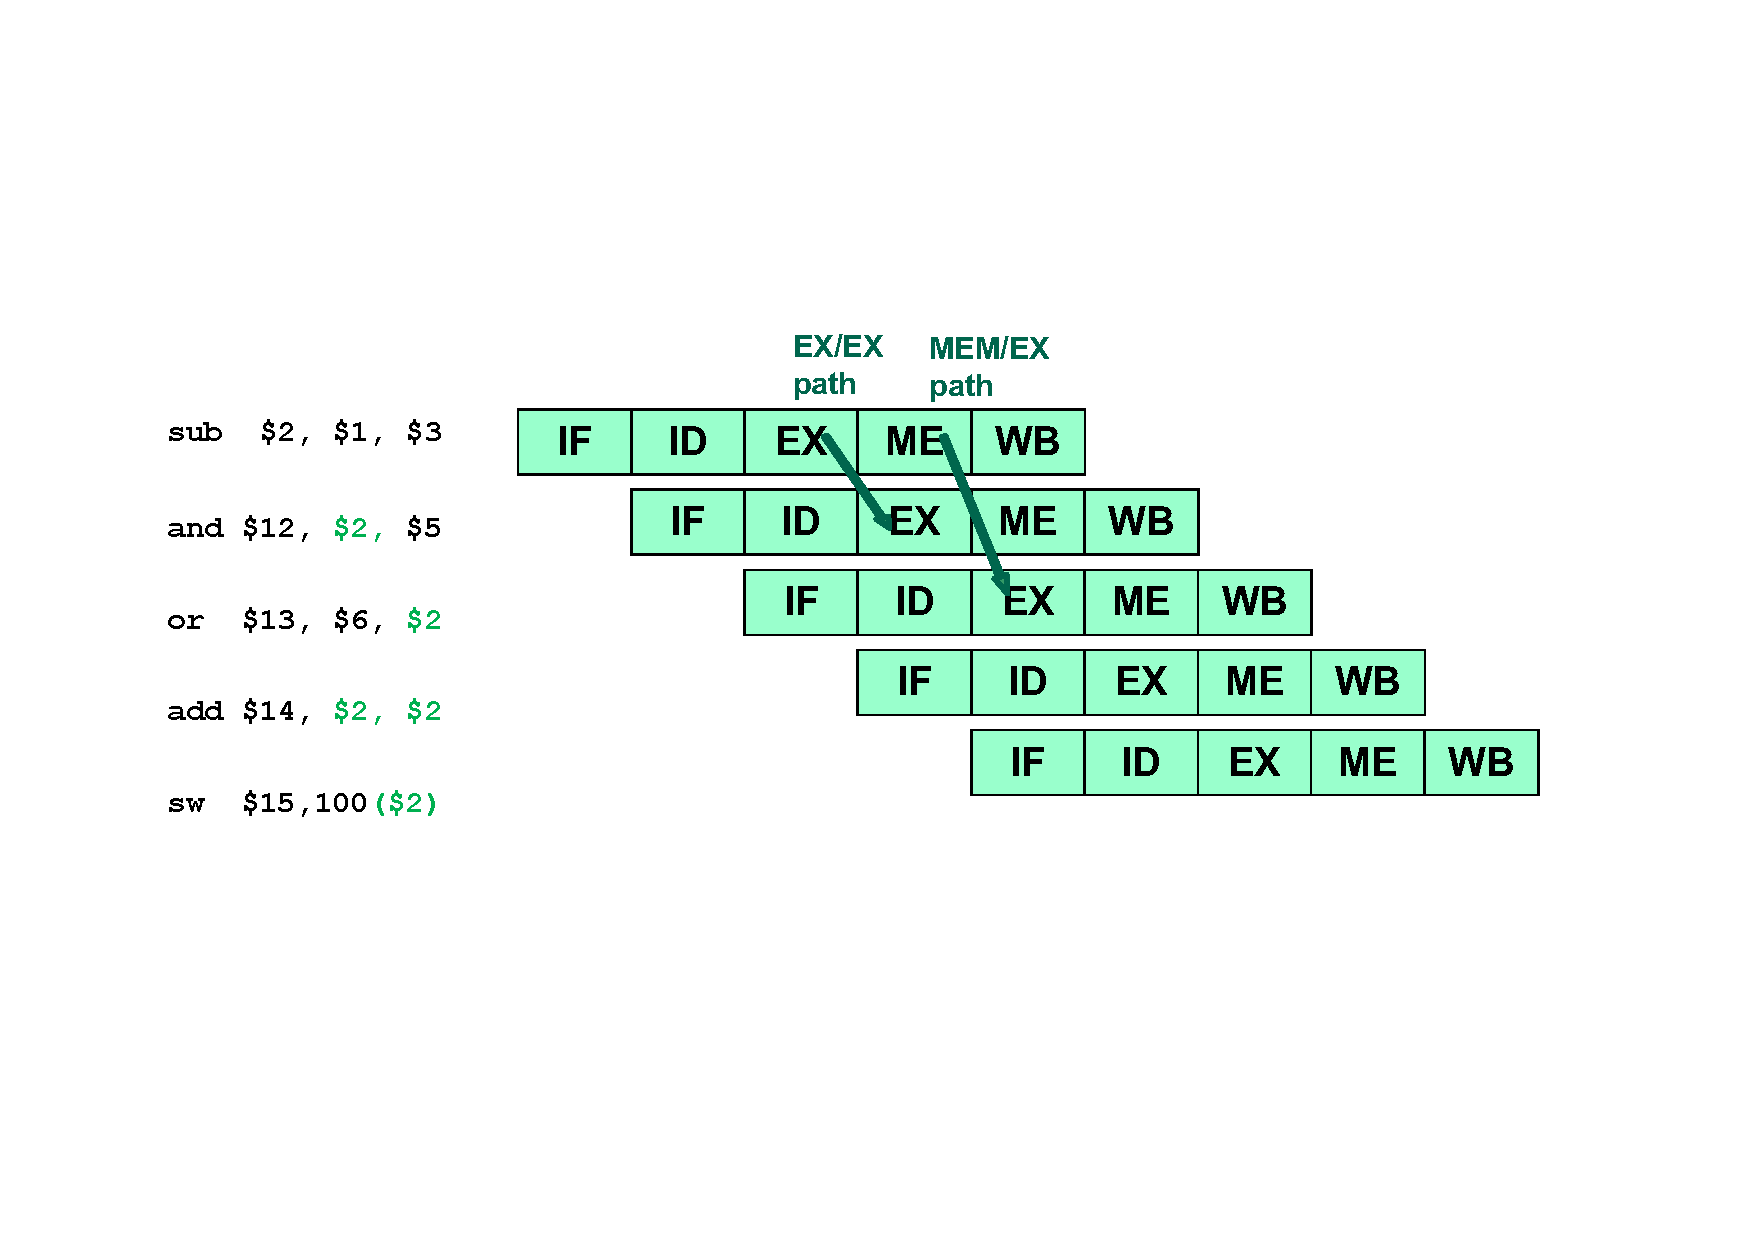
\includegraphics[width=\textwidth]{img/data-forwarding-1.pdf}
        \captionof*{figure}{Data forwarding.\cite{pipelining-slides}}
    \end{center}
\end{examplebox}
    \subsubsection{Performance evaluation in pipelining}

As we have seen in the previous sections, the \textbf{pipelining increases the CPU instruction throughput} (number of instructions completed per unit of time) but doesn't reduce the latency (the execution time of a single instruction).

\highspace
The \textbf{increase in latency is a direct consequence of two problems}:
\begin{itemize}
    \item The \indexdefinition{imbalance among the pipeline stages}

    \item The \indexdefinition{overhead in the pipeline control}
\end{itemize}
This imbalance between the pipeline stages and the overhead are \underline{bad aspects}:
\begin{itemize}
    \item The \textbf{imbalance} reduces performance because the \textbf{clock can run no faster than the time needed for the slowest pipeline stage};

    \item The \textbf{overhead} arises from the \textbf{delay introduced by interstage registers and clock skew}.
\end{itemize}
Finally, \textbf{all instructions should be the same number of pipeline stages}. Each assumption and optimization shown previously works well in this case.

\begin{definitionbox}[: number of Clock Cycles, Clocks Per Instructions and MIPS formula]
    Given:
    \begin{itemize}
        \item The \textbf{Instruction Count per iteration} as $\texttt{IC}_{\texttt{per\_iter}}$

        \item The \textbf{number of Stall Cycles per iteration} as \texttt{\# Stall Cycles}

        \item The \textbf{length of the pipeline} is $x$
    \end{itemize}
    We can \textbf{calculate the} \indexdefinition{number of Clock Cycles} as the sum between the Instruction Count (how many stages there are in one instruction), the number of Stall Cycles inserted by the hardware technique (called insertion of stalls), plus the length of the pipeline $x$:
    \begin{equation}\label{eq: clock cycles per iteration}
        \texttt{\# Clock Cycles}_{\texttt{per\_iter}} = \texttt{IC}_{\texttt{per\_iter}} + \texttt{\# Stall Cycles}_{\texttt{per\_iter}} + x
    \end{equation}
    The \indexdefinition{Clocks Per Instruction} per iteration, $\texttt{CPI}_{\texttt{per\_iter}}$, is calculated with the rapport between the number of Clock Cycles per iteration (previous equation) divided by the Instruction Count per iteration:
    \begin{equation}\label{eq: clock per instruction per iteration}
        \begin{array}{rcl}
            \texttt{CPI}_{\texttt{per\_iter}} &=& \dfrac{
                \texttt{\# Clock Cycles}_{\texttt{per\_iter}}
            }{
                \texttt{IC}_{\texttt{per\_iter}}
            } \\ \\
            &=& \dfrac{
                \left(\texttt{IC}_{\texttt{per\_iter}} + \texttt{\# Stall Cycles}_{\texttt{per\_iter}} + x\right)
            }{
                \texttt{IC}_{\texttt{per\_iter}}
            }
        \end{array}
    \end{equation}
    Finally, the \indexdefinition{MIPS formula} per iteration is calculated with the rapport between the frequency of the clock ($\texttt{f}_{\texttt{clock}}$) divided by the multiply between the Instructions Per Clock (as the ratio $1 \div \texttt{CPI}$) and $10^{6}$ (1 million instructions):
    \begin{equation}\label{eq: MIPS per iteration}
        \texttt{MIPS}_{\texttt{per\_iter}}
        =
        \dfrac{
            \texttt{f}_{\texttt{clock}}
        }{
            \left(
                \texttt{CPI}_{\texttt{per\_iter}} \times 10^{6}
            \right)
        }
    \end{equation}
\end{definitionbox}

\noindent
We can asymptotically (\texttt{AS}) rewrite equations \ref{eq: clock cycles per iteration}, \ref{eq: clock per instruction per iteration} and \ref{eq: MIPS per iteration} as follows:
\begin{equation}
    \texttt{\# Clock Cycles}_{\texttt{AS}} = \texttt{IC}_{\texttt{AS}} + \texttt{\# Stall Cycles}_{\texttt{AS}} + x
\end{equation}
\vspace{1em}
\begin{equation}
    \begin{array}{rcl}
        \texttt{CPI}_{\texttt{AS}} &=& \lim_{n \rightarrow \infty} \dfrac{
            \texttt{\# Clock Cycles}_{\texttt{AS}}
        }{
            \texttt{IC}_{\texttt{AS}}
        } \\ \\
        &=& \lim_{n \rightarrow \infty} \dfrac{
            \left(
                \texttt{IC}_{\texttt{AS}} + \texttt{\# Stall Cycles}_{\texttt{AS}} + x
            \right)
        }{
            \texttt{IC}_{\texttt{AS}}
        }
    \end{array}
\end{equation}
\vspace{1em}
\begin{equation}
    \texttt{MIPS}_{\texttt{AS}} = \dfrac{
        \texttt{f}_{\texttt{clock}}
    }{
        \left(\texttt{CPI}_{\texttt{AS}} \times 10^{6}\right)
    }
\end{equation}
Note: the \textbf{ideal speedup, then Clock Per Instruction, should be equal to 1}. But stalls cause the pipeline performance to degrade from the ideal performance, so we have the \indexdefinition{Average Clock Per Instruction (CPI)}:
\begin{equation}
    \begin{array}{rcl}
        \texttt{AVG}\left(\texttt{CPI}\right) &=& \texttt{Ideal CPI} + \texttt{\# Stall Cycles}_{\texttt{per\_instruction}} \\ \\
        &=& 1 + \texttt{\# Stall Cycles}_{\texttt{per\_instruction}}
    \end{array}
\end{equation}
And obviously, the \indexdefinition{Pipeline Stall Cycles per Instruction} is:
\begin{equation}
    \texttt{PSCI} = \texttt{Structural Haz.} + \texttt{Data Haz.} + \texttt{Control Haz.} + \texttt{Memory Stalls}
\end{equation}

    %%%%%%%%%%%%%%%%%%%%%%%%%%
    % Bibliography and index %
    %%%%%%%%%%%%%%%%%%%%%%%%%%
    \bibliography{bibtex}{}
\bibliographystyle{plain}

\newpage

\printindex
\end{document}